\documentclass[a4paper, 12pt]{article}

\usepackage[english]{babel}
\usepackage[utf8]{inputenc}
\usepackage{amsmath}
\usepackage{textcomp}
\usepackage{textgreek}
\usepackage{gensymb}
\usepackage{graphicx}
\usepackage{booktabs}
\usepackage[colorinlistoftodos]{todonotes}
\usepackage[left=2cm,right=2cm,top=2cm,bottom=2cm]{geometry}
\usepackage{comment}
\usepackage{multirow}
\usepackage{fancyhdr}
\usepackage[font=scriptsize,labelfont=bf]{caption}
\usepackage{wrapfig}
\usepackage{titlesec}
\usepackage{natbib}
\usepackage{setspace}

\definecolor{darkgray}{rgb}{0.3,0.3,0.3}

\pagestyle{fancy}
\fancyhf{}
\fancyhead[R]{
\includegraphics[scale = 0.07]{Logo_EPFL.png}}
\fancyhead[L]{\textcolor{darkgray}{Air Pollution \& Climate Change : Assignment 2}}
\fancyfoot[R]{\textcolor{darkgray}{\thepage}}
\fancyfoot[L]{\textcolor{darkgray}{Nikolai Orgland \& Antoine Spahr}}
 
\renewcommand{\headrulewidth}{0.5pt}
\renewcommand{\footrulewidth}{0.5pt}
\renewcommand{\familydefault}{\sfdefault}
 
\titleformat{\section}
 			{\large\bfseries\sffamily}
  			{\thesection}{1em}{}
\titleformat{\subsection}
 			{\small\bfseries\sffamily}
  			{\thesubsection}{1em}{}
\titleformat{\subsubsection}
 			{\small\slshape\sffamily}
			{\thesubsubsection}{1em}{}

\begin{document}
%------------------------------- Title Page ---------------------------------------
\thispagestyle{empty}
\begin{center}
    {\large ENV-400 Air Pollution and Climate Change}\\[0.2cm]
    
    {\normalsize Spring Semester 2019 }\\[1.2cm]
    
    \hrulefill 
    \\[0.5cm]
        {\Huge\textbf{Comparative analysis of air pollutants between Sion and Tänikon}}
    \\[0.5cm]
    \hrulefill 	
\end{center}

~\\[1.3cm]

\begin{center}
    
\includegraphics[scale=0.20]{Logo_EPFL.png}\\[1.5cm]
    {\large \today}\\[0.5cm]
\end{center}

~\\[2.3cm]

\begin{centering}
    \large
    Assignment Part 2 \\
\end{centering}

~\\[1.3cm]

\begin{centering}
    \large
    Nikolai \textsc{Orgland} \textit{\small nikolai.orgland@epfl.ch}\\ 
    Antoine \textsc{Spahr} \textit{\small antoine.spahr@epfl.ch}\\
\end{centering}

\vfill
\thispagestyle{empty} 

\pagenumbering{gobble}

%---------------------------------- Table of content -----------------------------
\newpage
\tableofcontents
\pagenumbering{gobble}
\newpage
\pagenumbering{arabic}
\setcounter{page}{1}

%------------------------------ text ----------------------------------------------

\section{Introduction}
    % present the scope of the analysis conducted in the second part 
    % tell again where the data are from 
    % what is the time period studied 
    % what locations
    
    In the \textit{Part 1} of the assignment on the comparative analysis of air pollutants, a descriptive analysis has been performed. The present report performs an inferential analysis to further compare the pollutant concentrations between Sion and Tänikon. The analyzed data has been provided by the National Air Pollution Monitoring Network (NABEL) of Switzerland. The data originates from two measurement stations pictured in figure \ref{location_fig} and contain measurements of O\textsubscript{3} [\textmu g/m\textsuperscript{3}], NO\textsubscript{2} [\textmu g/m\textsuperscript{3}], NO\textsubscript{x} [\textmu g/m\textsuperscript{3}] and PM10 [\textmu g/m\textsuperscript{3}], as well as temperature [\degree C], precipitation [mm/h] and radiation [W/m\textsuperscript{2}]. The data is supplemented with wind direction [\degree N] and wind speed [m/s] from MétéoSuisse. 
    \\
    \\
    The first station is located in Tänikon in the Canton of Thurgau at 583 meters above sea level in the North-Eastern part of Switzerland. The neighbouring area is rural with small villages and characterized by strongly fertilized grassland for cattle . The closest highway is located 4 km away from the station (See Figure \ref{location_fig} b).  \\
    \\
    The second station is located in Sion, the capital of the Canton of Valais in Southern Switzerland. This station is situated on the military airfield of Sion at 483 meters above sea level, about 2 km south-west of the city centre. Only 50 meters away, the highway A9 passes by the station with 35’000 cars per day. The station is furthermore located in the valley of the Rhône which lies in the heart of the Swiss Alps (see Figure \ref{location_fig} a). 
    \\
    \\
    The present work first assesses the differences in mean between week-end and week days for both pollutant and meteorological parameters. In particular, the potential presence of the so called week-end effect for ozone is checked. This effect is characterized by an increase in O\textsubscript{3} during the week-ends due to a decrease in NO\textsubscript{x} emissions. Our work then explores the correlation and lag correlation observed in the data. Thereafter, the nature of the emissions is defined for the month of July. Finally, an unusual period is analyzed.
    
    \begin{figure}[b]
        \centering
        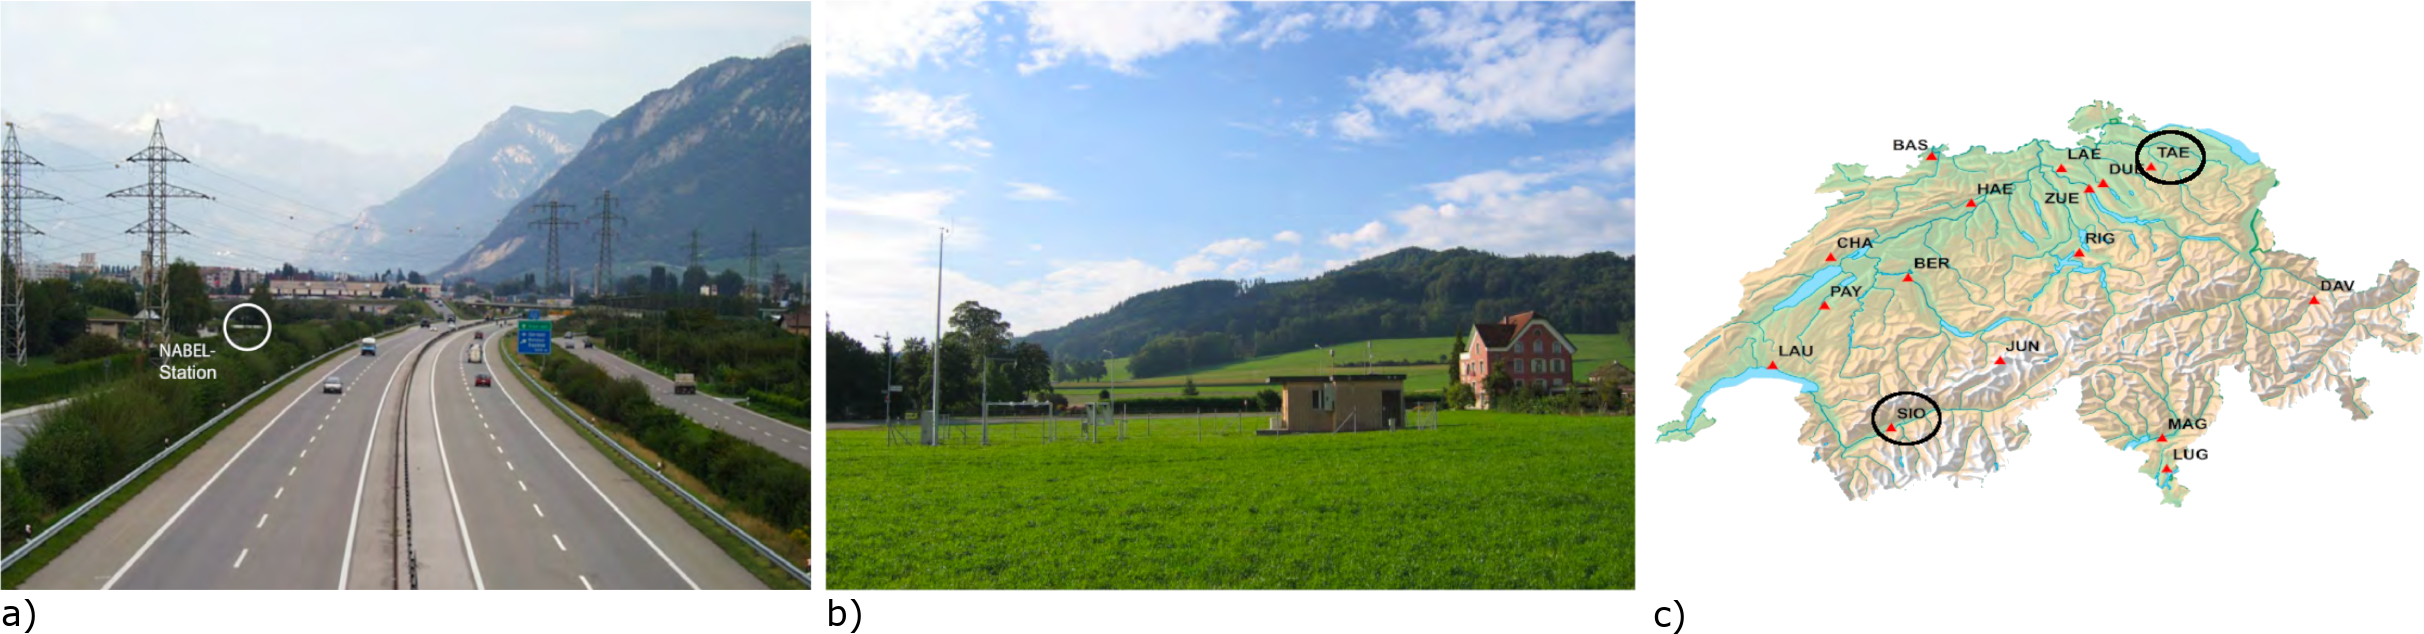
\includegraphics[width = 1 \textwidth]{Figures/Locations.png}
        \caption{\textbf{Measurement sites description.} Picture a) and b) respectively show the measurement site of Sion and Tänikon. Map c) shows the geographical situation of those two measurement stations (SIO and TAE) in Switzerland. They are highlighted with black circles. Source : \cite{NABEL}}
        \label{location_fig}
    \end{figure}
    
\section{Weekend vs Weekday} \label{sec:weekend}
    % present some expected differences 
    % present the graphs (data distribution, meadian, means) 
    % present the test and hypothesis used to compare means
    % present the p-vals 
    % conclude on significance 
    % discuss about the absence of ozone effects within locations
    Human activities such as transportation or household heating produce many emissions. However, the pollutants concentrations also changes with meteorological parameters. In order to grasp the effect of human activities on the pollutants concentrations, their distributions is observed separately between weekday and week-end. Indeed, human activities change considerably between those two parts of the week. In consequence, if the human activity has an impact on emissions, the emissions should be different during the weekdays. If human activity has no impact, emissions should not vary significantly during the weekdays and weekend. 
    \\
    \\
    The meteorological parameters (temperature, radiation, precipitation, wind speed and wind direction) should display similar distributions between week-day and week-end since they do not depend on the arbitrary distinction of week-end and week-day imposed by humans. However, the concentration of NO\textsubscript{2}, NO\textsubscript{x}, or PM10 are expected to be different between week-day and week-end since they are produced by human-induced combustion processes. The nitrogen bound in the fuel contributes to NO\textsubscript{x} emissions (so called fuel NO\textsubscript{2}). Furthermore, the heat generated by an engine converts some of the N\textsubscript{2} from the air into NO\textsubscript{2} (so-called thermal NO\textsubscript{x}). 
    \\
    \\
    O\textsubscript{3} formation relies on the photolysis of NO\textsubscript{2} to NO by liberating a mono-atomic oxygen atom that later can combine with diatomic oxygen to form O\textsubscript{3}. Ozone can then oxidize NO back into NO\textsubscript{2} and O\textsubscript{2}. Therefore there is a non-linear relationship between O\textsubscript{3} and NO\textsubscript{x}. The rate of ozone production also depends on the amount of volatile organic compounds (VOC) present in the air. Ozone concentrations can increase, decrease, or stay roughly constant for a change in NO\textsubscript{x} as presented on figure \ref{fig:ozoneScheme}. For a given concentration of VOC, if the concentration of NO\textsubscript{x} is low, ozone will be positively correlated with NO\textsubscript{x} (NO\textsubscript{x} sensitive zone). If NO\textsubscript{x} concentration is high, ozone will be negatively correlated with NO\textsubscript{x} (VOC-sensitive zone). And if NO\textsubscript{x} concentration is in between, there will be no strong correlation between ozone and NO\textsubscript{x}. In consequence, the presence of the so called week-end effect in ozone will depend on the NO\textsubscript{x} concentration. 
    \begin{figure}[t!]
        \centering
        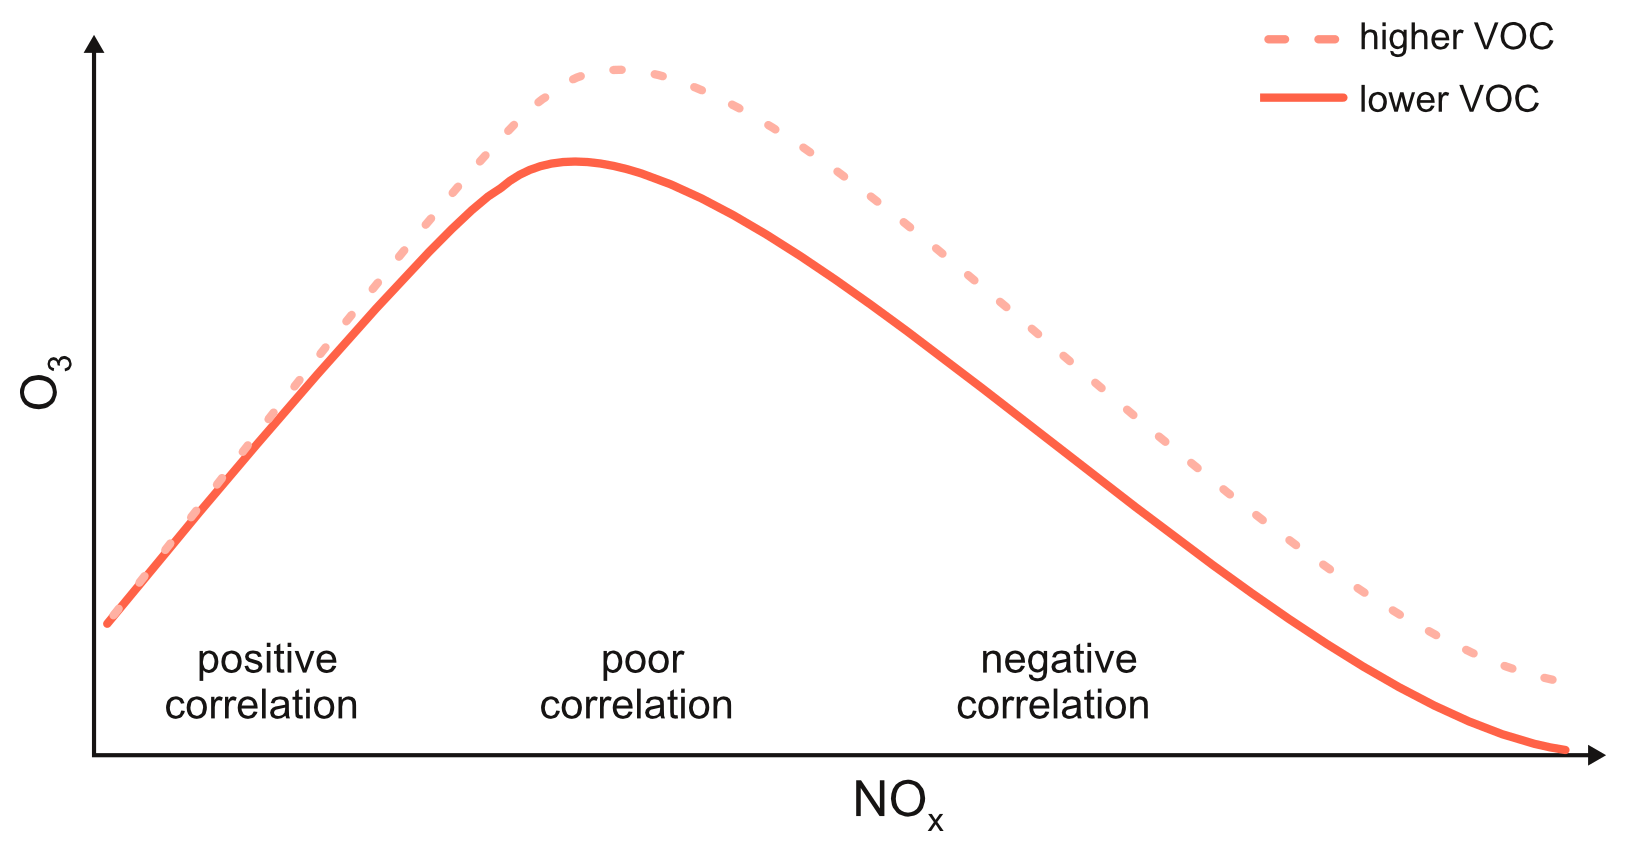
\includegraphics[width = 0.6 \textwidth]{Figures/O3vsNOx.png}
        \caption{\textbf{Scheme of ozone concentration in function of NO\textsubscript{x} and VOC.} The graphical scheme presents the non-linear relationship between ozone and NO\textsubscript{x} for two levels of VOC.}
        \label{fig:ozoneScheme}
    \end{figure}
    \begin{figure}[t!]
        \centering
        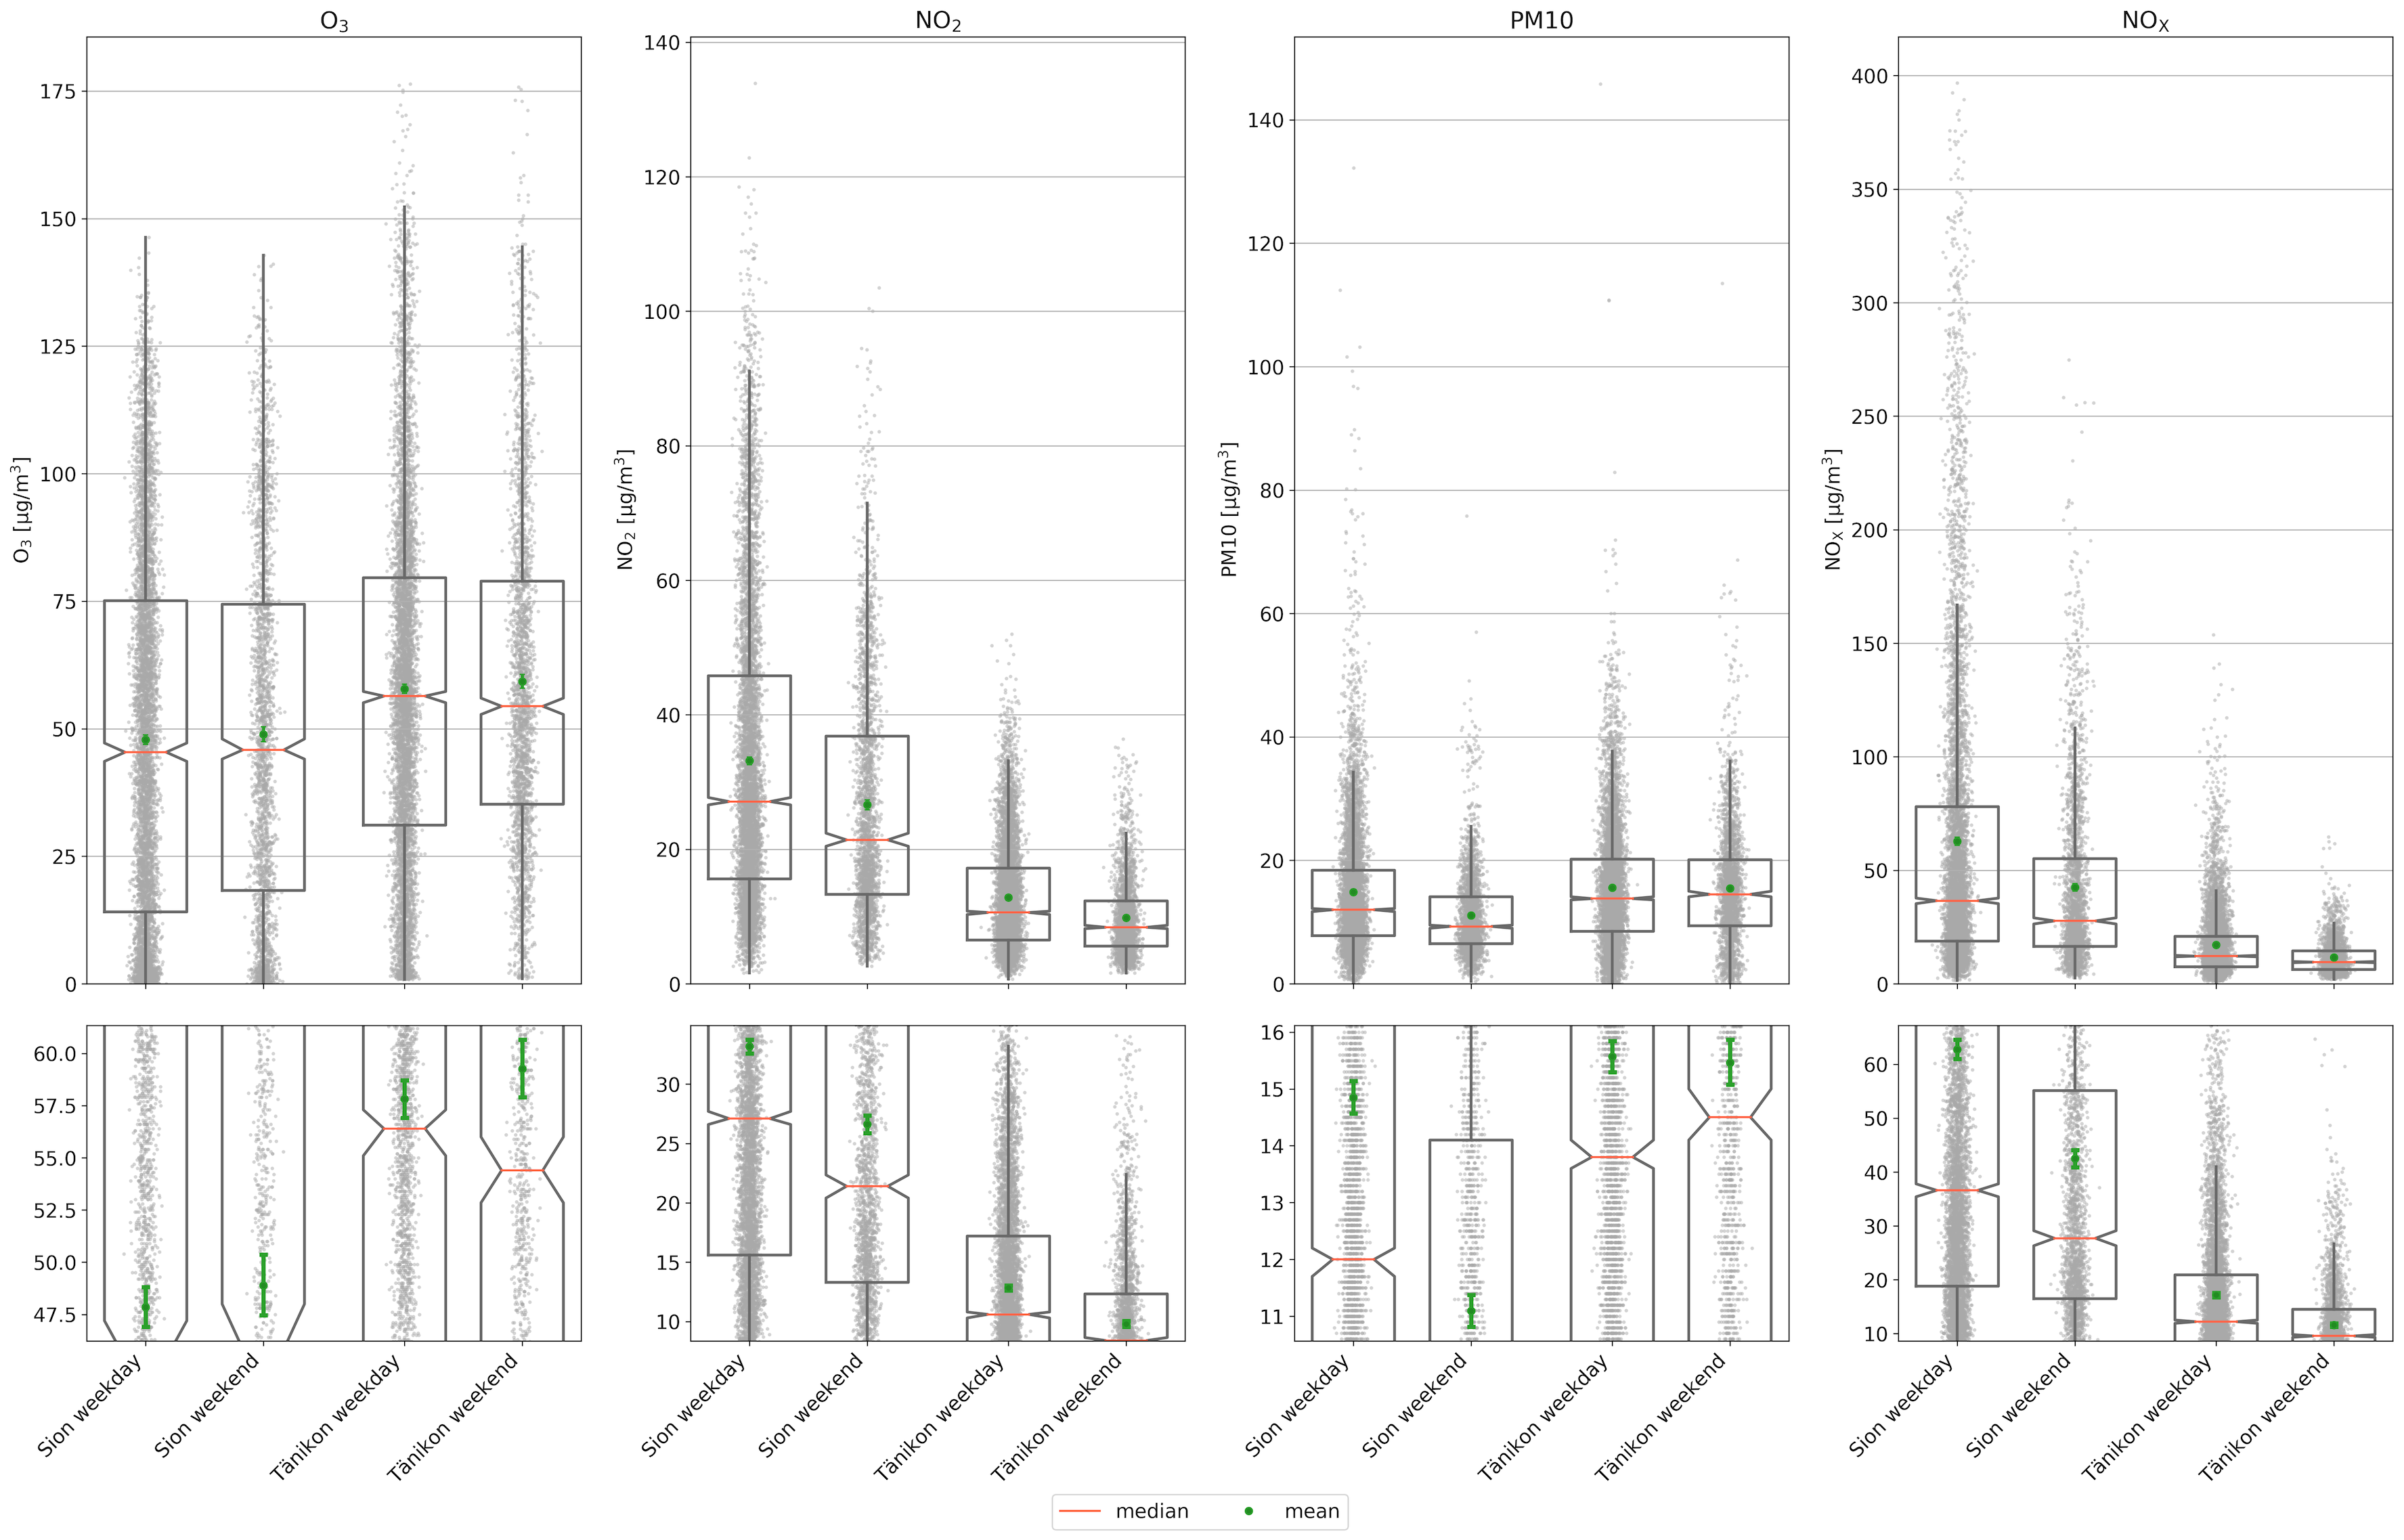
\includegraphics[width = 1 \textwidth]{Figures/boxplots_pollutants.png}
        \caption{\textbf{Pollutants concentrations boxplots by day type and locations.} The upper plots display the pollutants distributions. The notch on the box represents the 95\% confidence interval for the median. The lower plots provide a zoom on the means and their 95\% confidence intervals. Because the distribution are non normal, the confidence intervals for the mean have been computed by bootsrapping over 10'000 sampling.}
        \label{fig:pollutant_boxplot}
    \end{figure}
    \begin{figure}[t!]
        \centering
        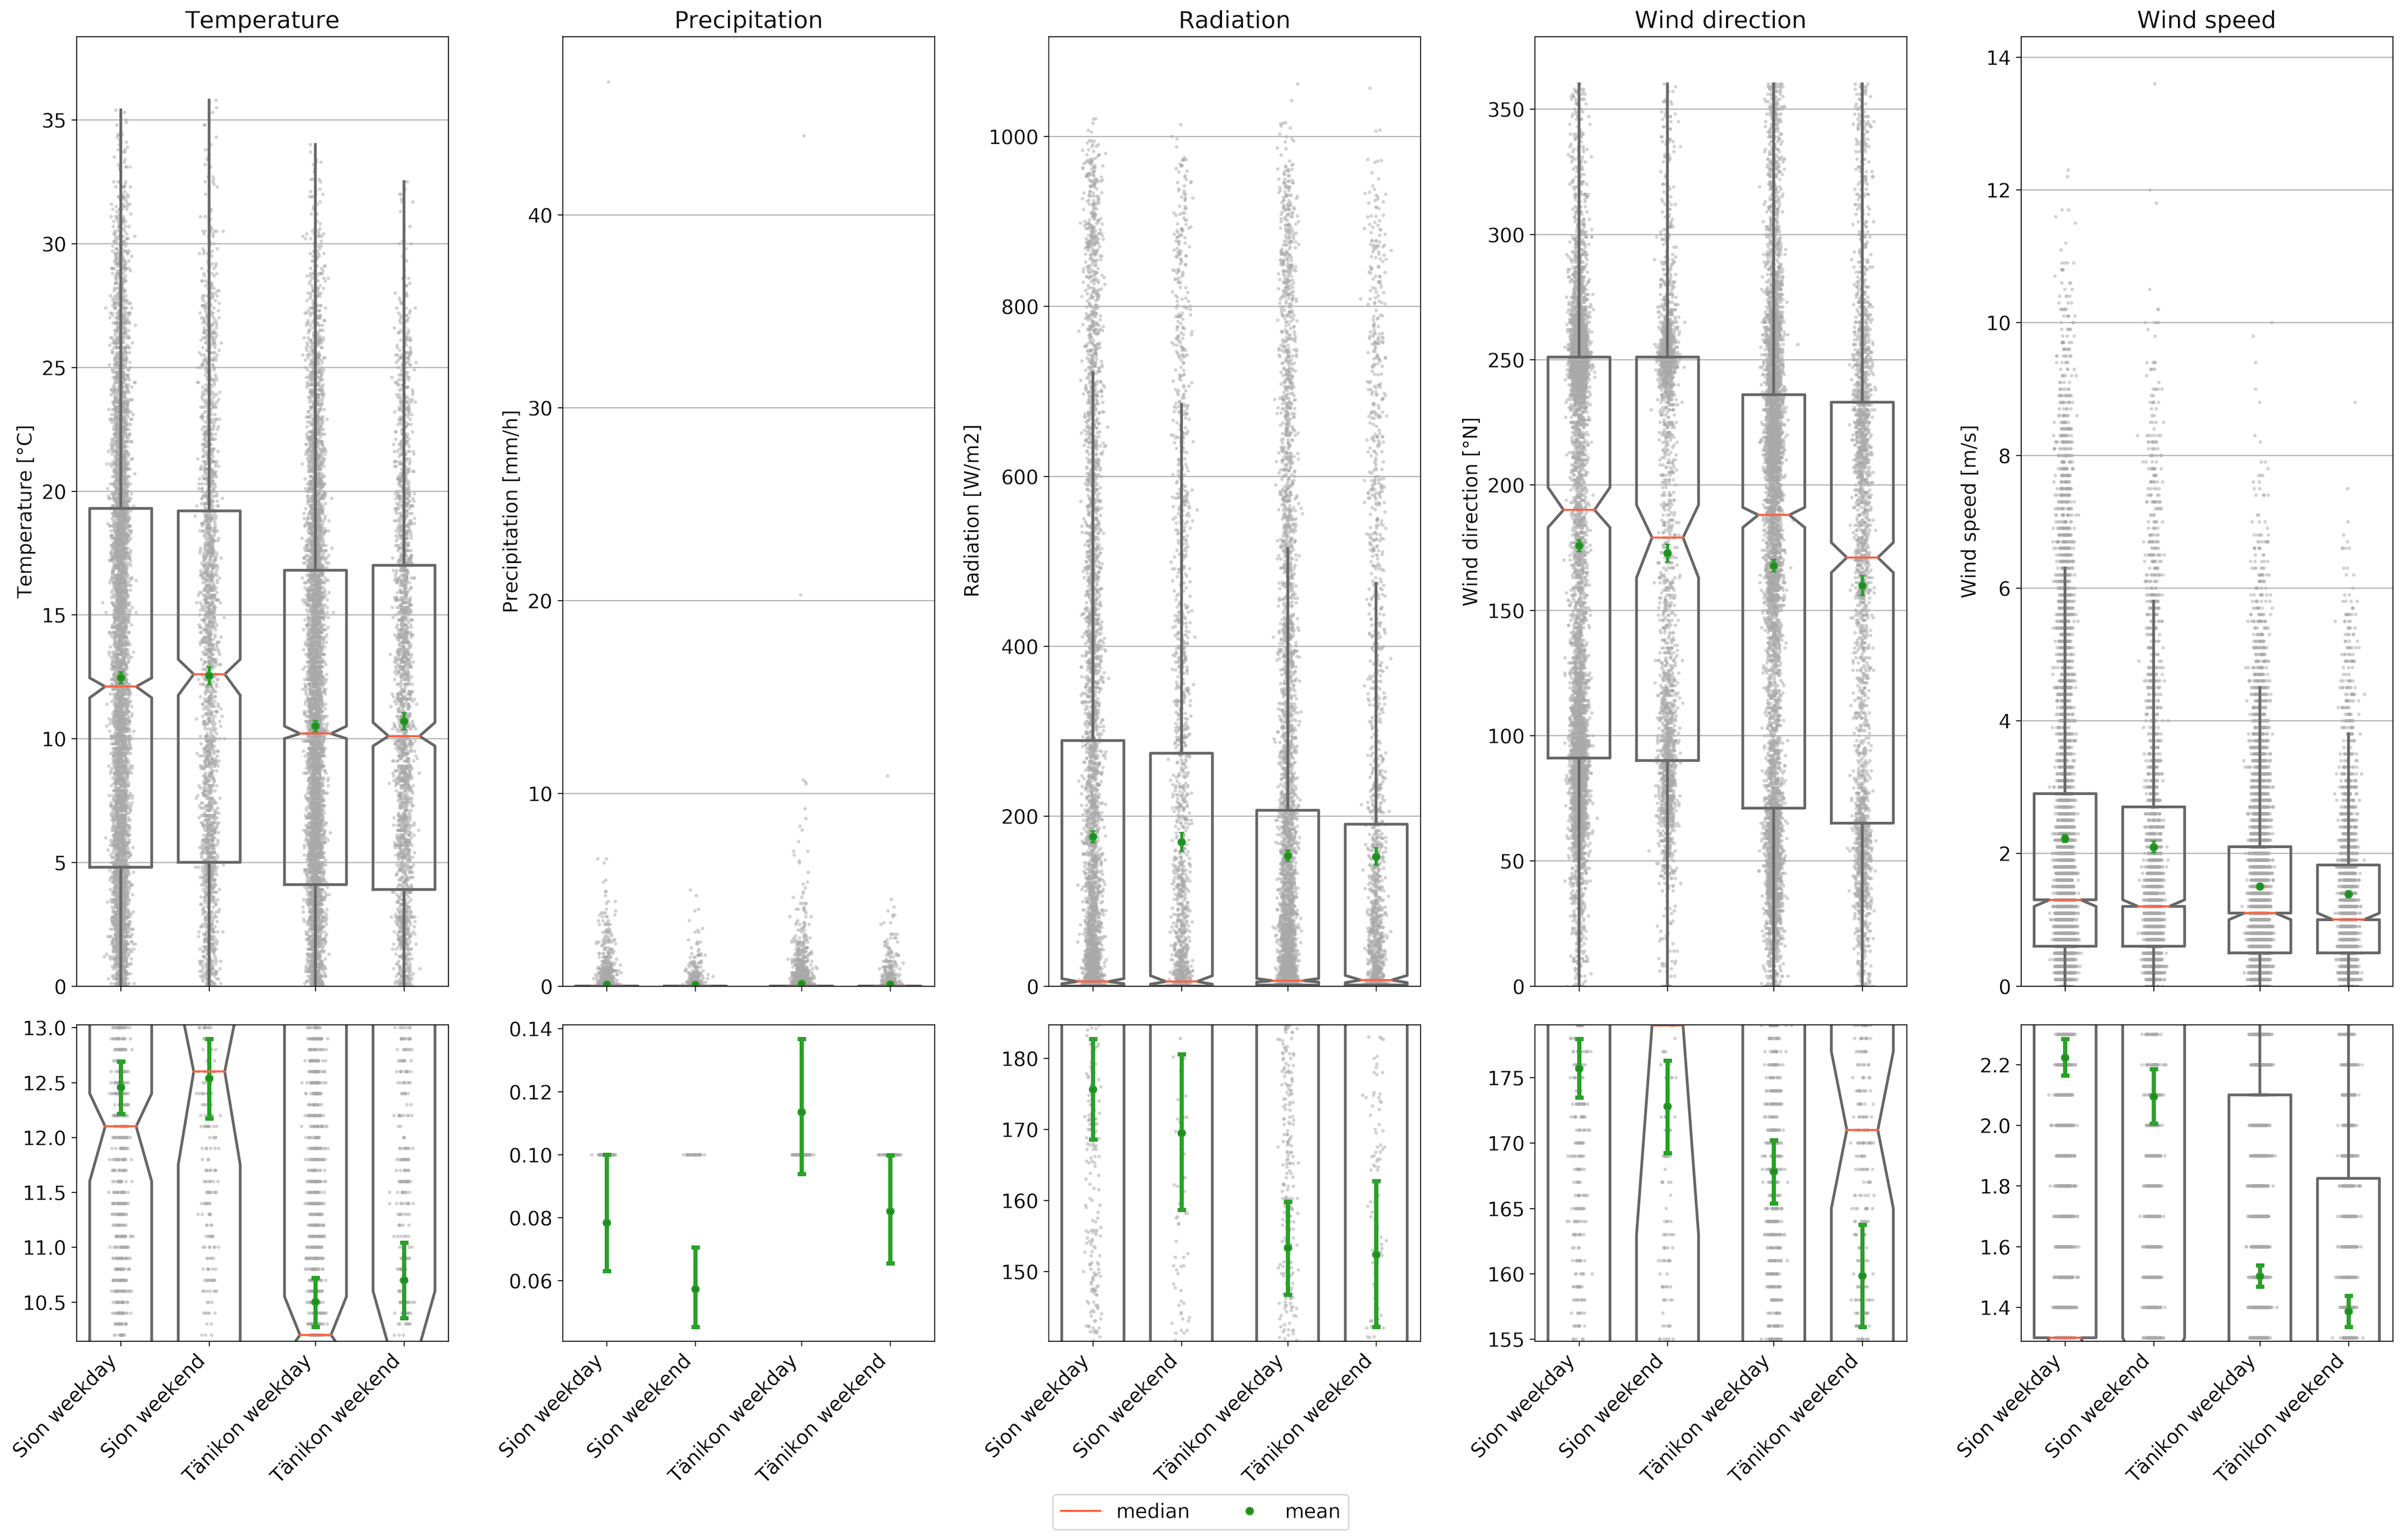
\includegraphics[width = 1 \textwidth]{Figures/boxplots_meteo.png}
        \caption{\textbf{Meteorological parameters boxplots by day type and locations.} The upper plots display the meteorological parameters distributions. The notch on the box represents the 95\% confidence interval for the median. The lower plots provide a zoom on the means and their 95\% confidence intervals. Because the distribution are non normal, the confidence intervals for the mean have been computed by bootsrapping over 10'000 sampling.}
        \label{fig:meteo_boxplot}
    \end{figure}
    \\
    \\
    In order to assess statistically the differences or similarities between week-end and week-day distributions as well as between the two locations, two series of tests have been conducted. Figure \ref{fig:pollutant_boxplot} and \ref{fig:meteo_boxplot} present respectively the distribution of pollutants and meteorological parameters for both locations on weekdays and week-ends. The lower parts of the figures are zooms on the means and the corresponding 95\% confidence-interval. \\
    \\
    The four samples means (week-end/weekday for Sion and Tänikon) are compared for each pollutant and meteorological parameter using a Mann-Whitney-U test. This test compares the means in a non-parametric fashion by confronting the null hypothesis \textit{H : the samples' means are similar} against the alternative hypothesis \textit{A : the sample's means are different}. The p-values obtained are presented on table \ref{tab:pval_mannwhitneyu}. The null hypotheses are rejected at a threshold of \textalpha = 5\%. These results are further confirmed when investigating the confidence intervals for the means presented on the lower plots of figure \ref{fig:pollutant_boxplot} and \ref{fig:meteo_boxplot} (the null hypothesis is rejected if the confidence intervals of the means do not overlap). 
    \\
    \begin{table}[b!]
        \caption{\textbf{P-values of the Mann-Whitney-U test.} The p-values highlighted in bold are the one significantly rejecting the null hypothesis \textit{H : the two samples means are similar} at a threshold of \textalpha = 5\%.}
        \label{tab:pval_mannwhitneyu}
        \resizebox{\textwidth}{!}{%
        \begin{tabular}{@{}lllllll@{}}
            \toprule
                           & \multicolumn{1}{c}{\begin{tabular}[c]{@{}c@{}}SIO weekday \\ vs \\ SIO weekend\end{tabular}} & \multicolumn{1}{c}{\begin{tabular}[c]{@{}c@{}}SIO weekday \\ vs \\ TAE weekday\end{tabular}} & \multicolumn{1}{c}{\begin{tabular}[c]{@{}c@{}}SIO weekday \\ vs \\ TAE weekend\end{tabular}} & \multicolumn{1}{c}{\begin{tabular}[c]{@{}c@{}}SIO weekend \\ vs \\ TAE weekday\end{tabular}} & \multicolumn{1}{c}{\begin{tabular}[c]{@{}c@{}}SIO weekend \\ vs \\ TAE weekend\end{tabular}} & \multicolumn{1}{c}{\begin{tabular}[c]{@{}c@{}}TAE weekday \\ vs \\ TAE weekend\end{tabular}} \\ \midrule
            O3             & 0.143                                                                                        & \textbf{5.22e-59}                                                                            & \textbf{8.21e-45}                                                                            & \textbf{9.12e-31}                                                                            & \textbf{5.18e-29}                                                                            & 0.108                                                                                        \\
            NO2            & \textbf{1.21e-33}                                                                            & \textbf{0}                                                                                   & \textbf{0}                                                                                   & \textbf{7.85e-310}                                                                           & \textbf{0}                                                                                   & \textbf{1.04e-51}                                                                            \\
            PM10           & \textbf{3.13e-58}                                                                            & \textbf{3.96e-15}                                                                            & \textbf{1.57e-12}                                                                            & \textbf{1.94e-101}                                                                           & \textbf{3.9e-84}                                                                             & 0.29                                                                                         \\
            NOX            & \textbf{4.28e-32}                                                                            & \textbf{0}                                                                                   & \textbf{0}                                                                                   & \textbf{7.94e-310}                                                                           & \textbf{0}                                                                                   & \textbf{2.07e-55}                                                                            \\
            Temperature    & 0.414                                                                                        & \textbf{2.24e-29}                                                                            & \textbf{3.02e-15}                                                                            & \textbf{9.96e-19}                                                                            & \textbf{5.86e-12}                                                                            & 0.239                                                                                        \\
            Precipitation  & 0.348                                                                                        & \textbf{5.22e-07}                                                                            & \textbf{0.000108}                                                                            & \textbf{3.73e-05}                                                                            & \textbf{0.00043}                                                                             & 0.459                                                                                        \\
            Radiation      & 0.346                                                                                        & \textbf{5.46e-83}                                                                            & \textbf{3.49e-50}                                                                            & \textbf{9.23e-50}                                                                            & \textbf{2.9e-36}                                                                             & 0.419                                                                                        \\
            Wind direction & 0.0963                                                                                       & \textbf{6.59e-21}                                                                            & \textbf{4.84e-27}                                                                            & \textbf{4.2e-09}                                                                             & \textbf{8.64e-16}                                                                            & \textbf{0.000269}                                                                            \\
            Wind speed     & 0.0543                                                                                       & \textbf{8.6e-43}                                                                             & \textbf{2.36e-37}                                                                            & \textbf{1.31e-18}                                                                            & \textbf{4.07e-21}                                                                            & \textbf{0.00371}                                                                             \\ \bottomrule
        \end{tabular}%
        }
    \end{table}
    \\
    The Mann-Whitney-U test failed to reject the null hypothesis for the meteorological parameters in the same location (Sion and Tänikon) except for the wind speed and direction in Tänikon. Those results confirmed our expectations as the meteorological parameters should not depend on the arbitrary week-end/week-day distinction. The difference in windspeed in Tänikon between week-end/week-day is probably arbitrary. On the other hand, the means are statistically different for all the meteorological parameters between Sion and Tänikon which confirm the climatic difference between the two stations. 
    \\
    \\
    In Sion the mean pollutant concentrations are statistically different between week-end and week-day for NO\textsubscript{2}, NO\textsubscript{x} and PM10. However, the ozone means are not significantly different between week-end and week-days. A similar pattern is observable in Tänikon with the exception of PM10 that is not significantly different between week-end and week-days. In addition, all the pollutant concentrations are significantly different between both locations, confirming the difference in local emissions. 
    \\
    \\
    In a second step, in order to assess the similarity of the overall distribution the four samples distributions, and not the mean. The data for  week-end/weekday for Sion and Tänikon are compared for each pollutant and meteorological parameter using a Kolmogorov-Smirnov test. This non parametric test compares the distribution of two samples by confronting the null hypothesis \textit{H : the samples come from the same distribution} against the alternative hypothesis \textit{A : the samples come from different distributions}. The p-values obtained are presented on table \ref{tab:pval_ks}. Similarly, the null hypotheses are rejected at a threshold of \textalpha = 5\%. Those results can be qualitatively confirmed by the distributions displayed on figure \ref{fig:pollutant_boxplot} for the air pollutants and on figure \ref{fig:meteo_boxplot} for the meteorological parameters. \\
    \\ 
    It appears that the distributions are significantly different between Sion and Tänikon, which confirm the similar results from the Mann-Whitney-U test. As expected, the Kolmogorov-Smirnov test does not yield significant differences in distribution for the meteorological parameters between week-end and week-days in both Sion and Tänikon, with the exception of the wind speed and wind direction in Tänikon. \\
    \\
    Contrary to the Mann-Whitney-U test, the Kolmogorov-Smirnov test yield significant differences between the ozone distribution in week-days and week-end both in Sion and Tänikon. However the results do not contradict each other. The results shows that the mean ozone concentrations are not significantly different while the underlying distributions clearly are. 
    \\
    \begin{table}[t!]
        \caption{\textbf{P-values of the Kolmogorov-Smirnov test.} The p-values highlighted in bold are the one significantly rejecting the null hypothesis \textit{H : samples come from the same distribution} at a threshold of \textalpha = 5\%.}
        \label{tab:pval_ks}
        \resizebox{\textwidth}{!}{%
        \begin{tabular}{@{}lllllll@{}}
            \toprule
            \multicolumn{1}{c}{} & \multicolumn{1}{c}{\begin{tabular}[c]{@{}c@{}}SIO weekday\\ vs\\ SIO weekend\end{tabular}} & \multicolumn{1}{c}{\begin{tabular}[c]{@{}c@{}}SIO weekday\\ vs\\ TAE weekday\end{tabular}} & \multicolumn{1}{c}{\begin{tabular}[c]{@{}c@{}}SIO weekday\\ vs\\ TAE weekend\end{tabular}} & \multicolumn{1}{c}{\begin{tabular}[c]{@{}c@{}}SIO weekend\\ vs\\ TAE weekday\end{tabular}} & \multicolumn{1}{c}{\begin{tabular}[c]{@{}c@{}}SIO weekend\\ vs\\ TAE weekend\end{tabular}} & \multicolumn{1}{c}{\begin{tabular}[c]{@{}c@{}}TAE weekday\\ vs\\ TAE weekend\end{tabular}} \\ \midrule
            O3                   & \textbf{0.0121}                                                                            & \textbf{1.28e-59}                                                                          & \textbf{1.71e-64}                                                                          & \textbf{2.2e-24}                                                                           & \textbf{1.14e-32}                                                                          & \textbf{2.35e-06}                                                                          \\
            NO2                  & \textbf{1.4e-22}                                                                           & \textbf{0}                                                                                 & \textbf{0}                                                                                 & \textbf{4.37e-207}                                                                         & \textbf{1.03e-305}                                                                         & \textbf{1.05e-43}                                                                          \\
            PM10                 & \textbf{1.62e-42}                                                                          & \textbf{3.76e-28}                                                                          & \textbf{2.37e-26}                                                                          & \textbf{2.8e-100}                                                                          & \textbf{7.64e-84}                                                                          & \textbf{0.0324}                                                                            \\
            NOX                  & \textbf{4.24e-23}                                                                          & \textbf{0}                                                                                 & \textbf{0}                                                                                 & \textbf{2.43e-240}                                                                         & \textbf{0}                                                                                 & \textbf{2.03e-42}                                                                          \\
            Temperature          & 0.327                                                                                      & \textbf{2.6e-31}                                                                           & \textbf{1.18e-16}                                                                          & \textbf{8.03e-17}                                                                          & \textbf{3.35e-11}                                                                          & 0.193                                                                                      \\
            Precipitation        & 1                                                                                          & \textbf{0.0425}                                                                            & \textbf{0.232}                                                                             & \textbf{0.143}                                                                             & \textbf{0.326}                                                                             & 1                                                                                          \\
            Radiation            & 0.722                                                                                      & \textbf{0}                                                                                 & \textbf{2.42e-321}                                                                         & \textbf{3.04e-313}                                                                         & \textbf{3.89e-226}                                                                         & 0.605                                                                                      \\
            Wind direction       & 0.137                                                                                      & \textbf{2.26e-78}                                                                          & \textbf{1.68e-53}                                                                          & \textbf{1.18e-38}                                                                          & \textbf{1.6e-32}                                                                           & \textbf{1.2e-05}                                                                           \\
            Wind speed           & 0.125                                                                                      & \textbf{1.05e-47}                                                                          & \textbf{2.76e-33}                                                                          & \textbf{1.48e-18}                                                                          & \textbf{1e-16}                                                                             & \textbf{0.000232}                                                                          \\ \bottomrule
            \end{tabular}%
        }
    \end{table}
    \\
    Finally, the study of the distributions between week-end and week-days of the air pollutants enables to highlight the presence of a week-end effect on NO\textsubscript{2} and NO\textsubscript{x} in both Sion and Tänikon. The concentrations of both are significantly lower during the week-end (see 95\% confidence intervals on figure \ref{fig:pollutant_boxplot}). Also the means of nitrogen dioxide are significantly different between week-end and week-days. This observation can be explained by the higher human activity during the week-days and the thus higher emissions. The week-end effect for O\textsubscript{3} is however less clear in both Sion and Tänikon. The means values for O\textsubscript{3} are not statistically different between week-days and week-end, whereas the distributions  are different. A slight increase in O\textsubscript{3} can be observed during the week-end in both Sion and Tänikon but it is not significant. The different outcomes of these two statistical tests may suggest that the weekend effect is quite small for ozone. As stated before, the rate of ozone production depends non-linearly on NO\textsubscript{x} and VOC concentration. In consequence, the dependency between NO\textsubscript{x} and O\textsubscript{3} seems to be between an absence of correlation and negative correlation (see figure \ref{fig:ozoneScheme}), leading to a small ozone increase during the week-end.
 
\section{Correlation}

    In the previous section \ref{sec:weekend}, statistical results have been linked to  physical processes in order to explained them. Hence, correlations between variables have been hypothesized and tested statistically. The present section explores in a deeper fashion inter-correlations between variables that may exist.
    \\
    \\
    The theoretical knowledge about the pollutant chemistry allows for making some hypotheses about which variables are expected to be correlated. First of all, NO\textsubscript{x} is a substance category that includes NO\textsubscript{2}. There should thus be a strong correlation between the two variables as they partially represent the same chemical substance. On another hand, NO\textsubscript{2} can be photolysed by solar radiation to free an atomic oxygen (O) that will then associate with O\textsubscript{2} to form O\textsubscript{3} \footnote{Note that the ozone production rate does not depend linearly on the nitrogen oxide concentration and different behaviour might be observed depending on the VOC concentration}. In consequence, one should expect nitrogen oxides to be negatively correlated with solar radiation as well as temperature (since a higher radiation often implies a higher temperature). In addition, NO\textsubscript{x} is expected to be negatively correlated with ozone. This comes from the supposition that the NO\textsubscript{x} concentration is in a negative correlation regime in both Sion and Tänikon (see figure \ref{fig:ozoneScheme}). However, as observed in section \ref{sec:weekend}, NO\textsubscript{x} and O\textsubscript{3} are in a state where no or only a slightly negative correlation is observed. Therefore, only a slight negative correlation is expected between them. Since O\textsubscript{3} production requires solar radiation, a positive correlation with radiation and temperature is expected. Moreover, precipitation may lower the PM10 concentration by capturing the particulate matter in the water droplets. Thus, a negative correlation between PM10 and the precipitation is expected. 
    
    \subsection{Correlation \& Lag correlation}
        In order to support or reject the previous hypothesis, the Pearson correlation coefficients between pairs of variables have been computed on hourly measures. However, since all the chemical processes do not happen instantaneously, there might be a lag between a change in a variable and the effect on another. This is why lag correlation has also been computed. The maximum correlation in absolute value is kept over 24 lags of 1h (12h before and 12h after). The correlations and lag correlations obtained for both locations are presented on figure \ref{fig:correlation_maps} as heat maps. 
        \\
        \begin{figure}[t!]
            \centering
            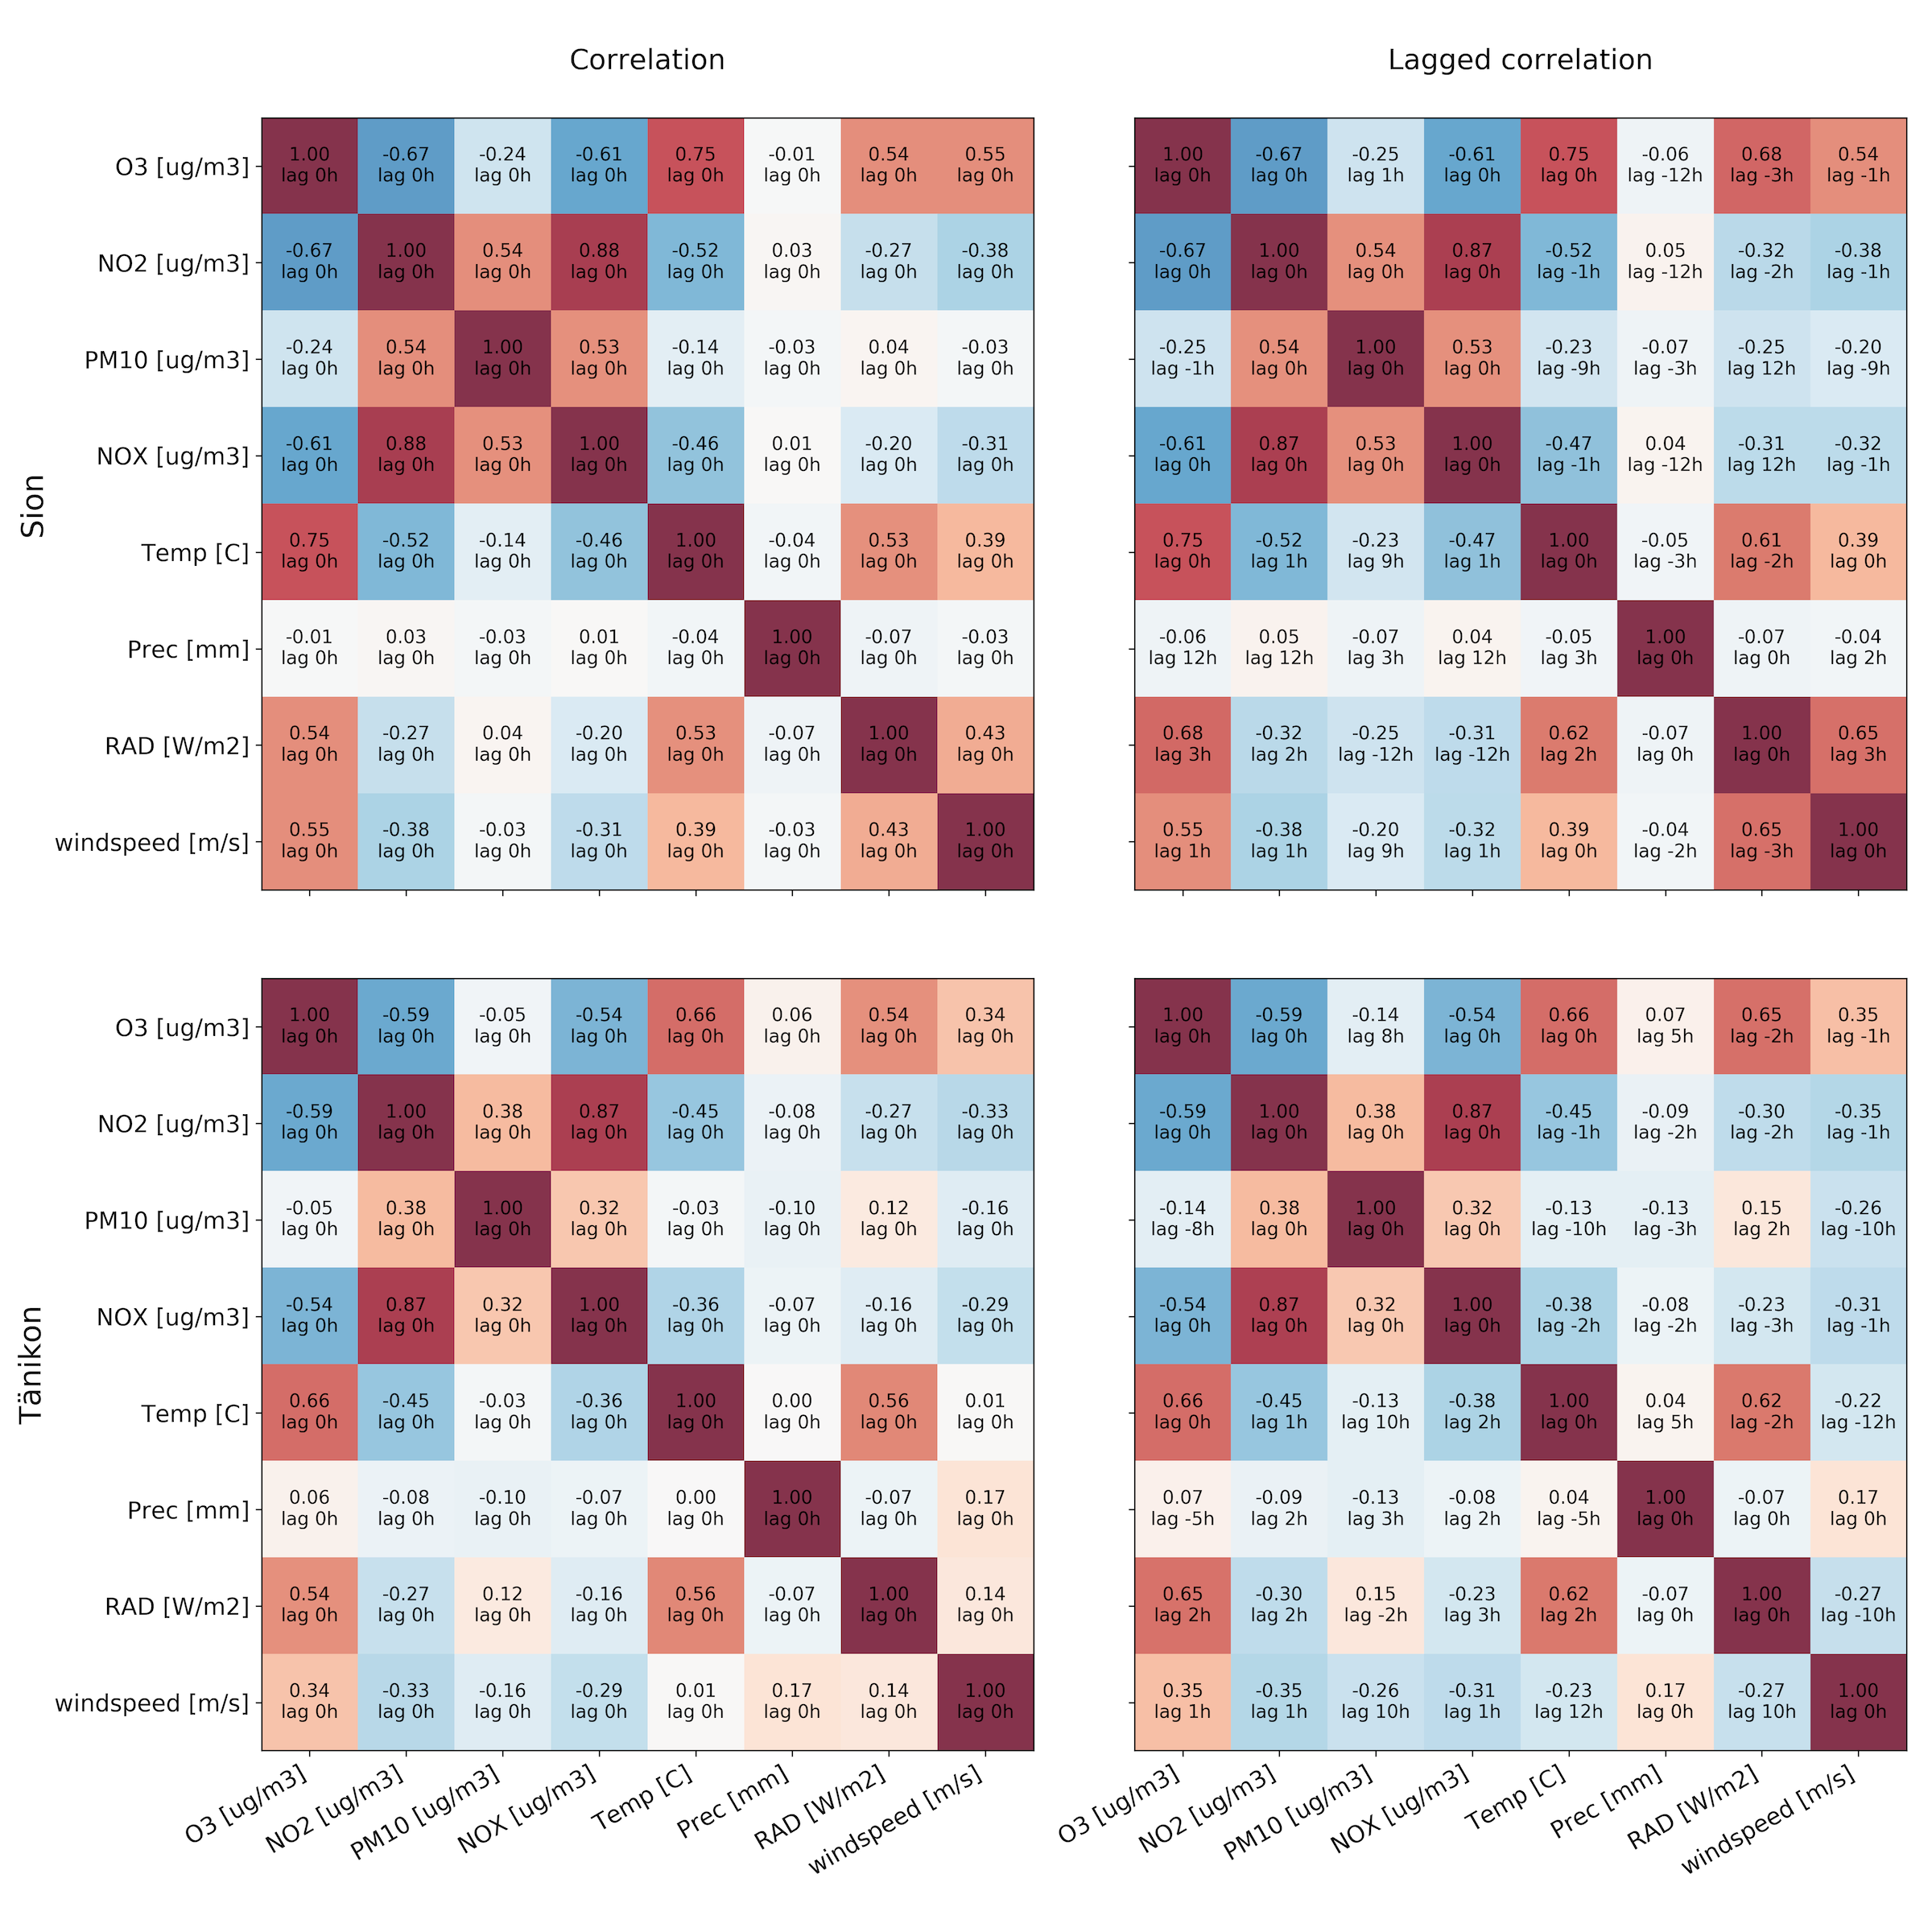
\includegraphics[width = 1 \textwidth]{Figures/yearly_correlations.png}
            \caption{\textbf{Correlation and lag-correlation between hourly pollutant concentrations and meteorological parameters.} The Pearson correlations between all the variables are presented as heat-maps. The color of the case corresponding to a pair of variables reflects the magnitude of correlation between them. A strong positive correlation will appear as dark red, whereas a strong negative correlation will appear as dark blue and an absence of linear correlation will appears as white. In addition to the color, the Pearson correlation coefficients are also displayed together with the lag yielding the highest correlation in absolute values. The lag tested ranges from 12h before to 12h after.}
            \label{fig:correlation_maps}
        \end{figure}
        \\
        It appears from the heat maps for Sion that O\textsubscript{3} is clearly positively correlated with temperature (0.75 with no lag) and radiation (0.68 with a lag of 3h). The lag of 3h changes the correlation from 0.54 to 0.68, highlighting the relevance of using lag correlations. A lag of 3h means that a change in radiation takes roughly 3h to show an effect on the ozone concentration. Furthermore, the correlation between the radiation and the temperature is maximum with a lag of 2h (correlation of 0.61). It thus means that it takes around 2h for the radiation to affect the temperature. As expected, ozone is negatively correlated with NO\textsubscript{2} and NO\textsubscript{x} (respectively -0.67 and -0.61 with no lag). The wind speed is also correlated with concentration of ozone (0.55 with a lag of 1h). The heat maps for Sion show that NO\textsubscript{2} and NO\textsubscript{x} are considerably positively correlated (0.87 with no lag). In addition, NO\textsubscript{2} is mildly negatively correlated with temperature and radiation (respectively -0.52 with a lag of 1h and -0.32 with a lag of 2h).
        \\
        However, the precipitation does not show any correlation with the other variables. This could be due to the large amount of data points with zero value (days with no rain). It means that the rainy events are quite sparse over time and a link between the variables cannot be observed with the correlations coefficient. \\
        \\
        The correlation patterns observed in Sion are similar to the ones observed in Tänikon. The lags yielding the strongest correlation between ozone and temperature/radiation are of similar order (respectively 0 and 2h). Nonetheless, the correlation coefficients between O\textsubscript{3} and temperature/radiation are slightly smaller in Tänikon than in Sion. 
        \\
        \\
        In brief, the data supports that NO\textsubscript{2} and NO\textsubscript{x} are correlated. NO\textsubscript{x} shows some negative correlation with ozone which indicates that we have a state where an increase in NO\textsubscript{x} induces a decrease in O\textsubscript{3}. In addition, the correlation between ozone, radiation and temperature also present the expected pattern : a clear positive correlation. The lag of 3h between the radiation peak and the ozone peak makes chemically sense as the ozone production is relatively slow. 
        \\
        However, the nitrogen oxides do not show the expected negative correlations with radiation. This is probably due to the rather large amount of zeros in the radiation samples (around half of the time) that represent the night measures. In consequence, NO\textsubscript{x} may fluctuate during the night while the radiation does not, which induces a reduction in correlation. 
        \\
        Moreover, the precipitation does not correlate with any other variable while a correlation with PM10 was expected. Similarly to the radiation case, it is likely due to the sparsity of precipitation events that does not allow the correlation to grasp the link between the two variables : PM10 can fluctuate a lot when there is no rain and thus the correlation tends towards zero if PM10 concentrations span over a large range for many time steps with no precipitation. It has been shown graphically (qualitatively) in the previous descriptive analysis (first assignment) that PM10 concentrations tend to drops during rain events. 
    
    \subsection{Seasonal changes in correlation} 
        \begin{figure}[t!]
            \centering
            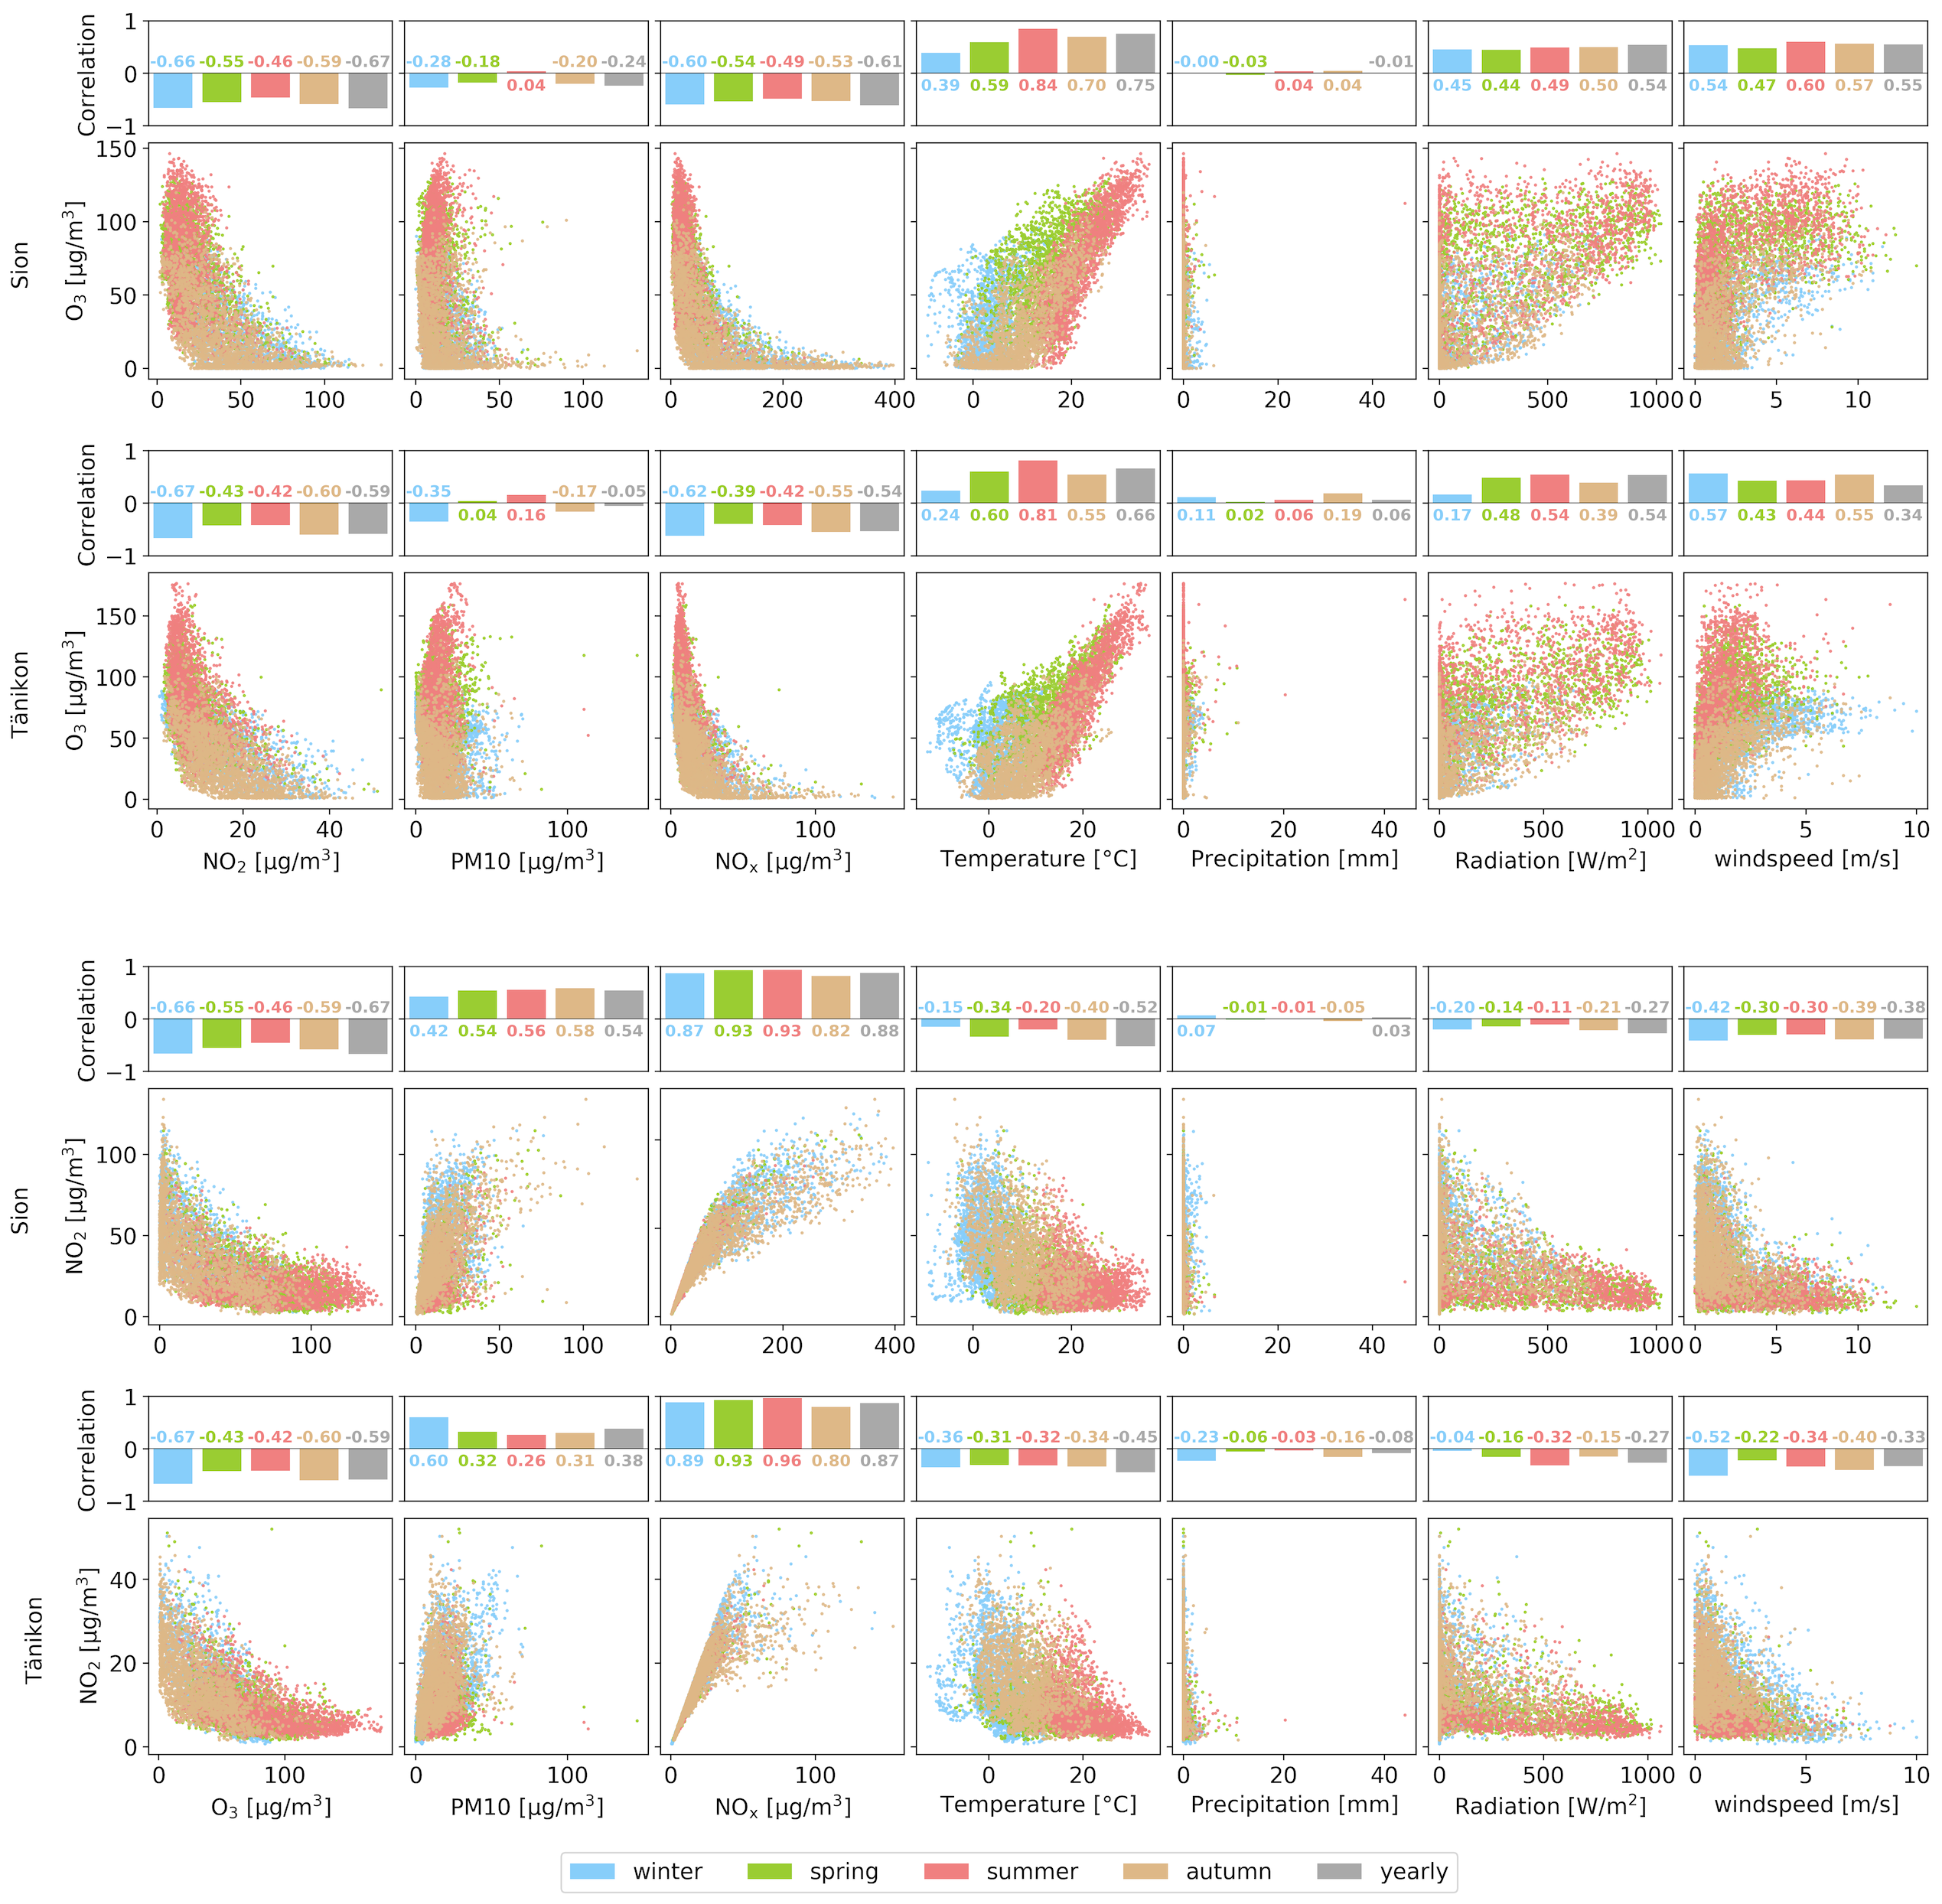
\includegraphics[width = 1 \textwidth]{Figures/scatter_hist_O3_NO2.png}
            \caption{\textbf{Scatter plots by season for O\textsubscript{3} and NO\textsubscript{2} against other variables.} For each variables pair, a histogram of Pearson's correlation coefficients by season is displayed on the top of the corresponding scatter-plot. The actual value of the correlation is displayed above/below the corresponding bar of the histogram. Note that the scatter-plot's axes are not scaled to the same range as only the pattern are compared.}
            \label{fig:scatter_hist}
        \end{figure}
        
        Computing only the correlation coefficient can leads to erroneous conclusions (as highlighted by the Anscombe's quartet) and to be sure that a relation exists, one should take a look at patterns of the scatter-plots. In addition, as most variables are dependent on meteorological parameters which are season dependant, the correlation between these variables is thus likely to be season dependant as well. To overcome these two limitations, the scatter plots between O\textsubscript{3} or NO\textsubscript{2} and the other variables have been made by season. The histogram of the corresponding correlation coefficients (without lag) are also added by season. The analysis focuses on O\textsubscript{3} and NO\textsubscript{2} because they are implied in most of the correlations pairs studied. The scatter-plots and the histograms by season are presented on figure \ref{fig:scatter_hist}.
        \\
        \\
        First, the scatter plots and correlations between Sion and Tänikon display similar patterns at different scales, except for the relation between NO\textsubscript{2} and PM10. In Sion, the correlation of PM10 with NO\textsubscript{2} is mild and roughly constant over the seasons, while in Tänikon the correlation is rather low except in winter where it reaches 0.60. The constant mild correlation in Sion could be due to the localization of the station (close to the highway) where PM10 and NO\textsubscript{2} are emitted together by the cars passing by (for example PM10 can be emitted by the car breaks rather than the car exaust). Since there is traffic on the highway all year round, the correlation is visible during all seasons. The correlation is not very high because PM10 can be emitted by many other sources such as pollen or dust lifted by the wind. Tänikon, on the other hand, is a more rural (village) station where the higher correlation between NO\textsubscript{2} and PM10 in winter could be due to the increased heating demand of households in the region. 
        \\
        \\
        Secondly, the strong correlation between O\textsubscript{3} and temperature or radiation is confirmed by the scatter plots. The correlation with temperature is higher during the summer, while the correlation with the radiation seems more constant through the year. The strong dependence with temperature is likely due to the underlying effect of radiation. Indeed figure \ref{fig:correlation_maps} shows that the most correlated lag between ozone and temperature is zero. The most correlated lag between ozone and radiation is 3h, while it is 2h between radiation and temperature. In consequence, the peak in temperature occurs roughly a the same time as the peak in O\textsubscript{3} and since the scatter plot displays non-lagged correlations, it would explain the better correlation between ozone and temperature. However it is still the radiation that causes the ozone production, but this can take some time. Nevertheless, the temperature can still have a direct effect on O\textsubscript{3} because a higher temperature may change the chemical rate constants and increase the rate of ozone production, which may explain as well the higher correlation with temperature during the summer.
        \\
        \\
        Third, the correlation between NO\textsubscript{x} and O\textsubscript{3} have a weak negative correlation. However, the scatterplot suggests that the dependency is not linear but rather as a $1/x$ function that would match the right part of the theoretical dependency between ozone and NO\textsubscript{x} presented in figure \ref{fig:ozoneScheme}. The scatterplot also visualizes the dependency that is not reflected in the correlation coefficients. This is because the Pearson coefficients reflects the linear dependency. In consequence, another metric, such as the Spearman coefficient, would be more suited for this case. The same pattern is observable between NO\textsubscript{2} and O\textsubscript{3} but in a noisier fashion. 
        \\
        As expected, the scatterplots confirm the high correlation between NO\textsubscript{2} and NO\textsubscript{x} over the four seasons since one is included in the other.
        \\
        \\
        The ozone has some weak positive correlations with the wind speed on both locations for all seasons. On the other hand, NO\textsubscript{2} has a weak negative correlation with the wind speed. The scatterplot further suggest that a high wind speed is associated with low concentrations of NO\textsubscript{2}. A possible explanation of the correlation between ozone and wind speed could be the increase of atmospheric mixing of NO\textsubscript{2} (which is of often a point source). A better dispersion of nitrogen oxides may increase the possibilities to react with light and produce ozone which thus increases with wind speed. Another explanation could be the transportation of pollutants from other locations towards or away from the measuring sites. 
        \\
        \\
        To sum up, the scatterplots and Pearson correlation coefficients by season do not only confirm the correlations observed previously but also enable to grasp the actual relationship. Indeed, based on the correlation coefficient the relation between NO\textsubscript{2} and O\textsubscript{3} exists, but the scatterplot shows that the relation does not look linear. In addition the scatterplots allow to observe the effect of the season on the correlations. In summer the correlation between ozone and temperature are higher because of the increased radiation. Overall, the pattern seems similar between Sion and Tänikon. 

\section{Emissions' nature} \label{emission_type}

    How the pollutants are emitted can have an influence on the understanding of the data and how they are interpreted. In consequence, to study the nature of the emissions (point emission or diffusive emission), the hourly and daily pollutants concentrations distributions are compared to log-normal distributions. First the data are transformed by taking the logarithm and then the resulting sample is tested for normality using a D'Agostino-K\textsuperscript{2} test which confronts the null hypothesis \textit{H : the distribution is Gaussian}, against the alternative hypothesis \textit{A: the distribution is not Gaussian}. In consequence, a fail to reject the null hypothesis would mean that the sample is log-normally distributed. If the null hypothesis is rejected, then the sample does not follow a log-normal distribution. The null hypothesis is rejected with a threshold of \textalpha = 5\%. The p-values obtained are presented on table \ref{tab:pval_log_normal_test} for both locations. 
    \\
    \begin{table}[t]
        \begin{minipage}{0.48\textwidth}
            \caption{\textbf{P-values of the D'Agostino-K\textsuperscript{2} test for normality.} The p-values highlighted in bold are the one significantly rejecting the null hypothesis \textit{H : the sample is normally distributed} at a threshold of \textalpha = 5\%.}
            \label{tab:pval_log_normal_test}
            \resizebox{\textwidth}{!}{%
            \begin{tabular}{@{}llllll@{}}
                \toprule
                                     & \multicolumn{2}{c}{hourly}                             &  & \multicolumn{2}{c}{daily}                              \\ \cmidrule(lr){2-3} \cmidrule(l){5-6} 
                                     & \multicolumn{1}{c}{Sion} & \multicolumn{1}{c}{Tänikon} &  & \multicolumn{1}{c}{Sion} & \multicolumn{1}{c}{Tänikon} \\ \midrule
                O\textsubscript{3}   & \textbf{5.49e-34}        & \textbf{1.2e-19}            &  & 0.196                    & 0.158                       \\
                NO\textsubscript{2}  & 0.441                    & \textbf{1.36e-06}           &  & 0.134                    & 0.208                       \\
                PM10                 & \textbf{5.34e-4}         & \textbf{7.65e-11}           &  & 0.452                    & 0.0513                      \\
                NO\textsubscript{X}  & \textbf{0.00551}         & \textbf{6.88e-05}           &  & 0.156                    & 0.307                       \\ \bottomrule
            \end{tabular}%
            }
        \end{minipage}%
        \hfill
        \begin{minipage}{0.50\textwidth}
            \caption{\textbf{P-values of the Shapiro-Wilk test for normality.} The p-values highlighted in bold are the one significantly rejecting the null hypothesis \textit{H : the sample is normally distributed} at a threshold of \textalpha = 5\%.}
            \label{tab:pval_shapiro}
            \resizebox{\textwidth}{!}{%
            \begin{tabular}{@{}llllll@{}}
            \toprule
                                 & \multicolumn{2}{c}{hourly}                             &  & \multicolumn{2}{c}{daily}                              \\ \cmidrule(lr){2-3} \cmidrule(l){5-6} 
                                 & \multicolumn{1}{c}{Sion} & \multicolumn{1}{c}{Tänikon} &  & \multicolumn{1}{c}{Sion} & \multicolumn{1}{c}{Tänikon} \\ \midrule
            O\textsubscript{3}   & \textbf{5.38e-24}        & \textbf{1.77e-15}           &  & 0.0745                   & 0.086                       \\
            NO\textsubscript{2}  & 0.0701                   & \textbf{5.19e-05}           &  & \textbf{0.0229}          & 0.0785                      \\
            PM10                 & \textbf{2.56e-05}        & \textbf{1.87e-08}           &  & 0.219                    & \textbf{0.0038}             \\
            NO\textsubscript{X}  & \textbf{4.87e-4}         & \textbf{5.99e-06}           &  & \textbf{0.0229}          & 0.206                       \\ \bottomrule
            \end{tabular}%
            }
        \end{minipage}%
    \end{table}
    \\
    First of all it appears from the p-values obtained that on hourly measurements only NO\textsubscript{2} in Sion fails to reject the null-hypothesis (p-values = 0.441). However, for daily values all the pollutants for both locations fail to reject the null hypothesis. 
    \\
    \\
    It is important to notice that the D’Agostino K\textsuperscript{2} test is suited for large samples (N $>$ 50 \cite{RalphB1990}) and since the focus is on the month of July, the sample of daily values is composed of only 31 samples. In consequence, the p-values obtained on daily values might not be relevant. This is why also a Shapiro-Wilk test is performed. The Shapiro-Wilk test is suited for small samples. In consequence it might not be suited for hourly values. The Shapiro-Wilk test confronts the same null and alternative hypothesis as the D’Agostino-K\textsuperscript{2} test. The results of the Shapiro-Wilk test are presented on table \ref{tab:pval_shapiro}.
    \\
    All hourly samples reject the null hypothesis except for NO\textsubscript{2} in Sion. For the daily values, only PM10 in Tänikon, NO\textsubscript{2} and NO\textsubscript{x} in Sion reject the null hypothesis. 
    \\
    Consequently, the results of both tests suggest that hourly NO\textsubscript{2} in Sion is log-normally distributed, while all the other hourly samples are not. On the other hand, most of the daily samples seems to be log-normally distributed. Daily nitrogen oxides in Sion and daily PM10 in Tänikon may not be log-normally distributed according to the Shapiro-Wilk test. 
    \\
    \begin{figure}[t!]
        \centering
        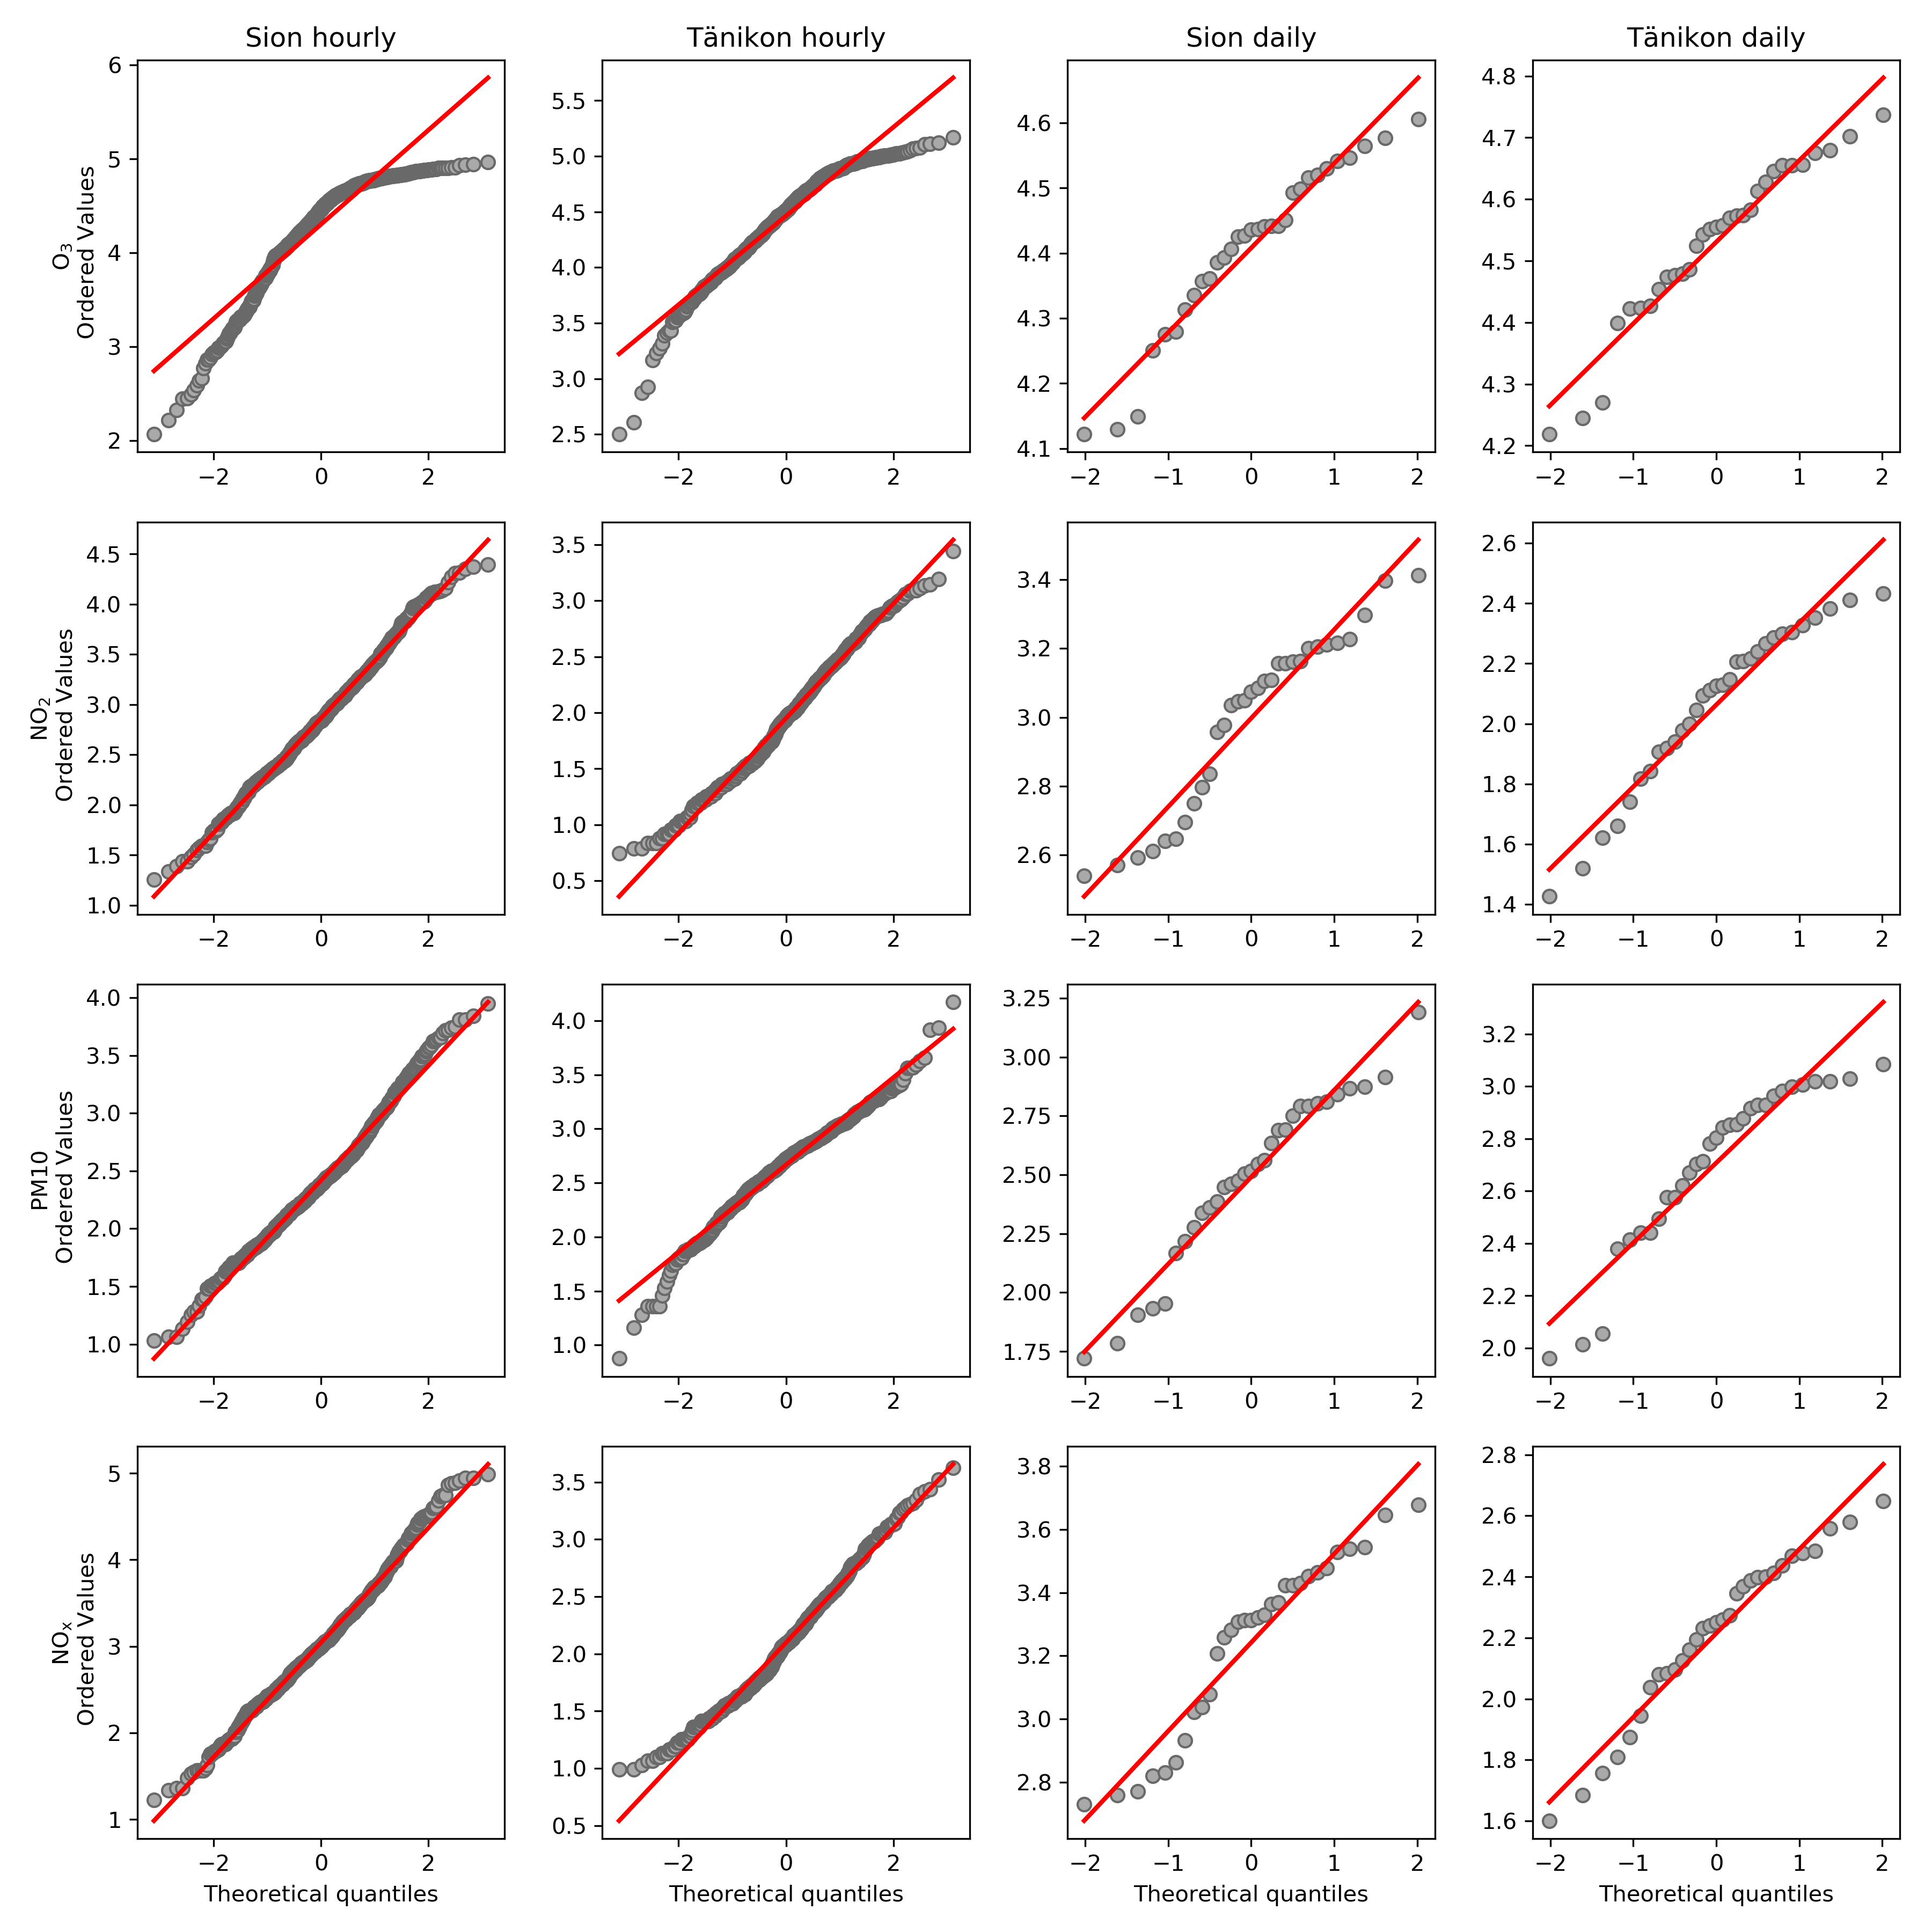
\includegraphics[width = 1 \textwidth]{Figures/QQplots.png}
        \caption{\textbf{QQ-plots for the logarithm of the pollutants concentrations.} The QQ-plot is computed on the logarithm of the pollutants concentrations for both hourly and daily measure of July, on both locations (Sion and Tänikon).}
        \label{fig:QQ-plots}
    \end{figure}
    \\
    To understand what a log-normal distribution implies, a point/local particles emission is considered. If the volume (the atmosphere) is discretized into multiple cells, then the diffusion of the particles from one cell to a neighbouring one is a random process and the amount of particles ending in the adjacent cell follows a normal distribution. In consequence, the amount of particles in a cell further away would results from a series of diffusion from a cell to the other and is thus the product of multiple random processes (from cell 1 to cell 2, from cell 2 to cell 3, and so on until the considered cell is reached). As a result, the log of the particle concentrations is a sum of normally distributed variables and the concentration is thus log-normally distributed. 
    \\ 
    Therefore, a point/local emission would result in a log-normal distribution of the concentration at the measurement site (further away from the source). However if the emission is not punctual/local, the distribution would not be log-normally distributed as the concentration at the measurement point would depend on a more homogeneous source. 
    \\
    \\
    A visual impression of the normality of the log-concentrations is presented on figure \ref{fig:QQ-plots} thanks to QQ-plots. \\
    \\ 
    First of all, in the hourly samples in Sion only NO\textsubscript{2} appears to be log-normally distributed and thus only NO\textsubscript{2} seems to be a point source of emission. Indeed the measurement stations is not situated directly on the highway, but close by. The highway may thus appear as a point source for NO\textsubscript{2}. However, one would have expected NO\textsubscript{x} to be log-normally distributed as well - but this is not the case. The QQ-plot check suggest that there are more large values of NO\textsubscript{x} than what a normal distribution would indicate. This could explain the outcome of the test for NO\textsubscript{x} in Sion : the sample is large and thus a small deviation from the normal is sufficient to reject the null hypothesis. In overall, NO\textsubscript{2} and NO\textsubscript{x} QQ-plots looks quite alike.
    \\
    It make sense the that nitrogen oxides are point sources in Sion station as they are mainly produced by car engines and the NABEL station is close to the highway (see figure \ref{location_fig}). 
    \\
    \\
    Secondly, the normality tests as well as the QQ-plots demonstrate that on both locations, O\textsubscript{3} is not log-normally distributed and is thus not emitted as a point source. This results makes sense as ozone is dependant on photo-chemistry (photolysis of nitrogen oxides) that may occur in multiple places in the atmospheric layer at once (where there is solar radiation) producing multiple sources around the measurement stations. 
    \\
    \\
    At hourly measurements, the statistical test indicates that PM10 does not seems to be emitted by point sources on both locations. However the QQ-plots suggests that the PM10 concentration is close to normality in Sion but not in Tänikon. In consequence,  PM10 could be emitted as a point source in Sion but not in Tänikon. A possible cause for this results is the presence of a gravel quarry south-west (positions: 46.211N ; 7.329E) of the Sion measurement station (around 1.5 km away), coupled with wind principally coming from south-west. Consequently, the gravel quarry produces dust (PM10) that is carried in the direction of the NABEL station. However other dust emissions sources may produce the non-normalities inducing the rejection of test's null-hypothesis. On the other hand, there is also a gravel quarry around 2 km north of the Tänikon NABEL station. However in July, the wind direction is mainly coming from the south. Therefore, the dust is carried away from the measurement station. That may explain why the PM10 is not log-normally distributed in Tänikon.
    \\
    \\
    The outcome of the Shapiro-Wilk test on daily averages (table \ref{tab:pval_shapiro}) appears to be different than on hourly averages. Indeed, all the pollutants fail to reject the null hypothesis which were expected for NO\textsubscript{2} and NO\textsubscript{x} in Sion and PM10 in Tänikon. Note that the D’Agostino K\textsuperscript{2} test fails to reject the null hypothesis for all pollutant in both locations, but since this test is not suited for small sized samples (less than 50) those results are not considered and the focus is given to the Shapiro-Wilk test results. 
    \\
    By looking at the daily average distribution, one gets insight on the pollutant concentration at a lower temporal resolution. Hence, the changes observed represent changes over longer time periods. Therefore, if a sample is log-normally distributed on daily averages, it would mean that the pollutant's emission can be considered as a point source on the long term.
    \\
    It turns out that NO\textsubscript{2} and NO\textsubscript{x} in Sion as well as PM10 in Tänikon are not log-normally distributed. It means that these emissions cannot be seen as point sources for a daily resolution in July. With the Shapiro-Wilk test, the other pollutants (ozone, PM10 in Sion as well as NO\textsubscript{x} and NO\textsubscript{2} in Tänikon) and can however been seen as point sources on a daily evolution. 
    \\
    \\
    The surprising number of point source patterns for the daily values in July could be explained by air pollutants that may move with the wind in a constant direction and are perceived as a point source at the measurement station. Nitrogen oxide in Sion are mainly coming from the cars passing b, and since the regime is changing between week-end and week days, it may be causing the absence of log-normal distribution on a daily basis. On the other hand, the qq-plots for the daily values (see figure \ref{fig:QQ-plots}) present some sort of patters deviating from the normal distribution for all pollutants. It could be that none of them are really log-normally distributed but the Shapiro-Wilk's test simply fails to reject the null hypothesis and thus sees the potential deviation as noise only.
        
\section{Unusual pattern}

    PM10 concentration in Tänikon gravitates around 10-20 [\textmu g/m\textsuperscript{3}]. The mean PM10 concentration in Tänikon over the year is ~15 [\textmu g/m\textsuperscript{3}]. Few hourly measures go over 40 [\textmu g/m\textsuperscript{3}] and the daily mean rarely exceeds 40 [\textmu g/m\textsuperscript{3}]. As a matter of fact, daily PM10 concentration in Tänikon exceed 40 [\textmu g/m\textsuperscript{3}] during seven days through the year 2018. Four of those seven days occurred in a rather continuous time interval between February and March (22.02.2018 ; 28.02.2018 ; 01.03.2018 ; 04.03.2018). In consequence, a time period spanning from the 17.02.018 to the 09.03.2018 is considered for the following analysis and refereed as \textit{unusual period}. 
    \\
    \\
    First of all, a one-tailed Mann-Whitney-U test is performed to assess whether the PM10 mean concentration during the unusual period is higher than the mean over the winter season. It thus tests : \textit{H : \textmu \textsubscript{PM10 unusual period} = \textmu \textsubscript{PM10 winter}} against \textit{A : \textmu \textsubscript{PM10 unusual period} $>$ \textmu \textsubscript{PM10 winter}}. The null hypothesis is significantly rejected with a p-value of 2.314$\cdot$10\textsuperscript{-126}. Therefore, the PM10 concentration in Tänikon during the unusual period is significantly higher. That is why it is considered unusual in this analysis. 
    \\
    \\
    The top left plot of figure \ref{fig:unusual-summary-plots} presents the diurnal evolution of the four days during which the daily PM10 exceed 40 [\textmu g/m\textsuperscript{3}]. It appears that the PM10 concentration is almost always above 40 [\textmu g/m\textsuperscript{3}]. Therefore, the high daily concentration of PM10 is not due to a punctual high concentration (outlier) but to a constant high concentration. In consequence, it does not seem to be a measurement anomaly and a further analysis to understand why the PM10 concentration was high during this period is required.
    \\
    \begin{figure}[t]
        \centering
        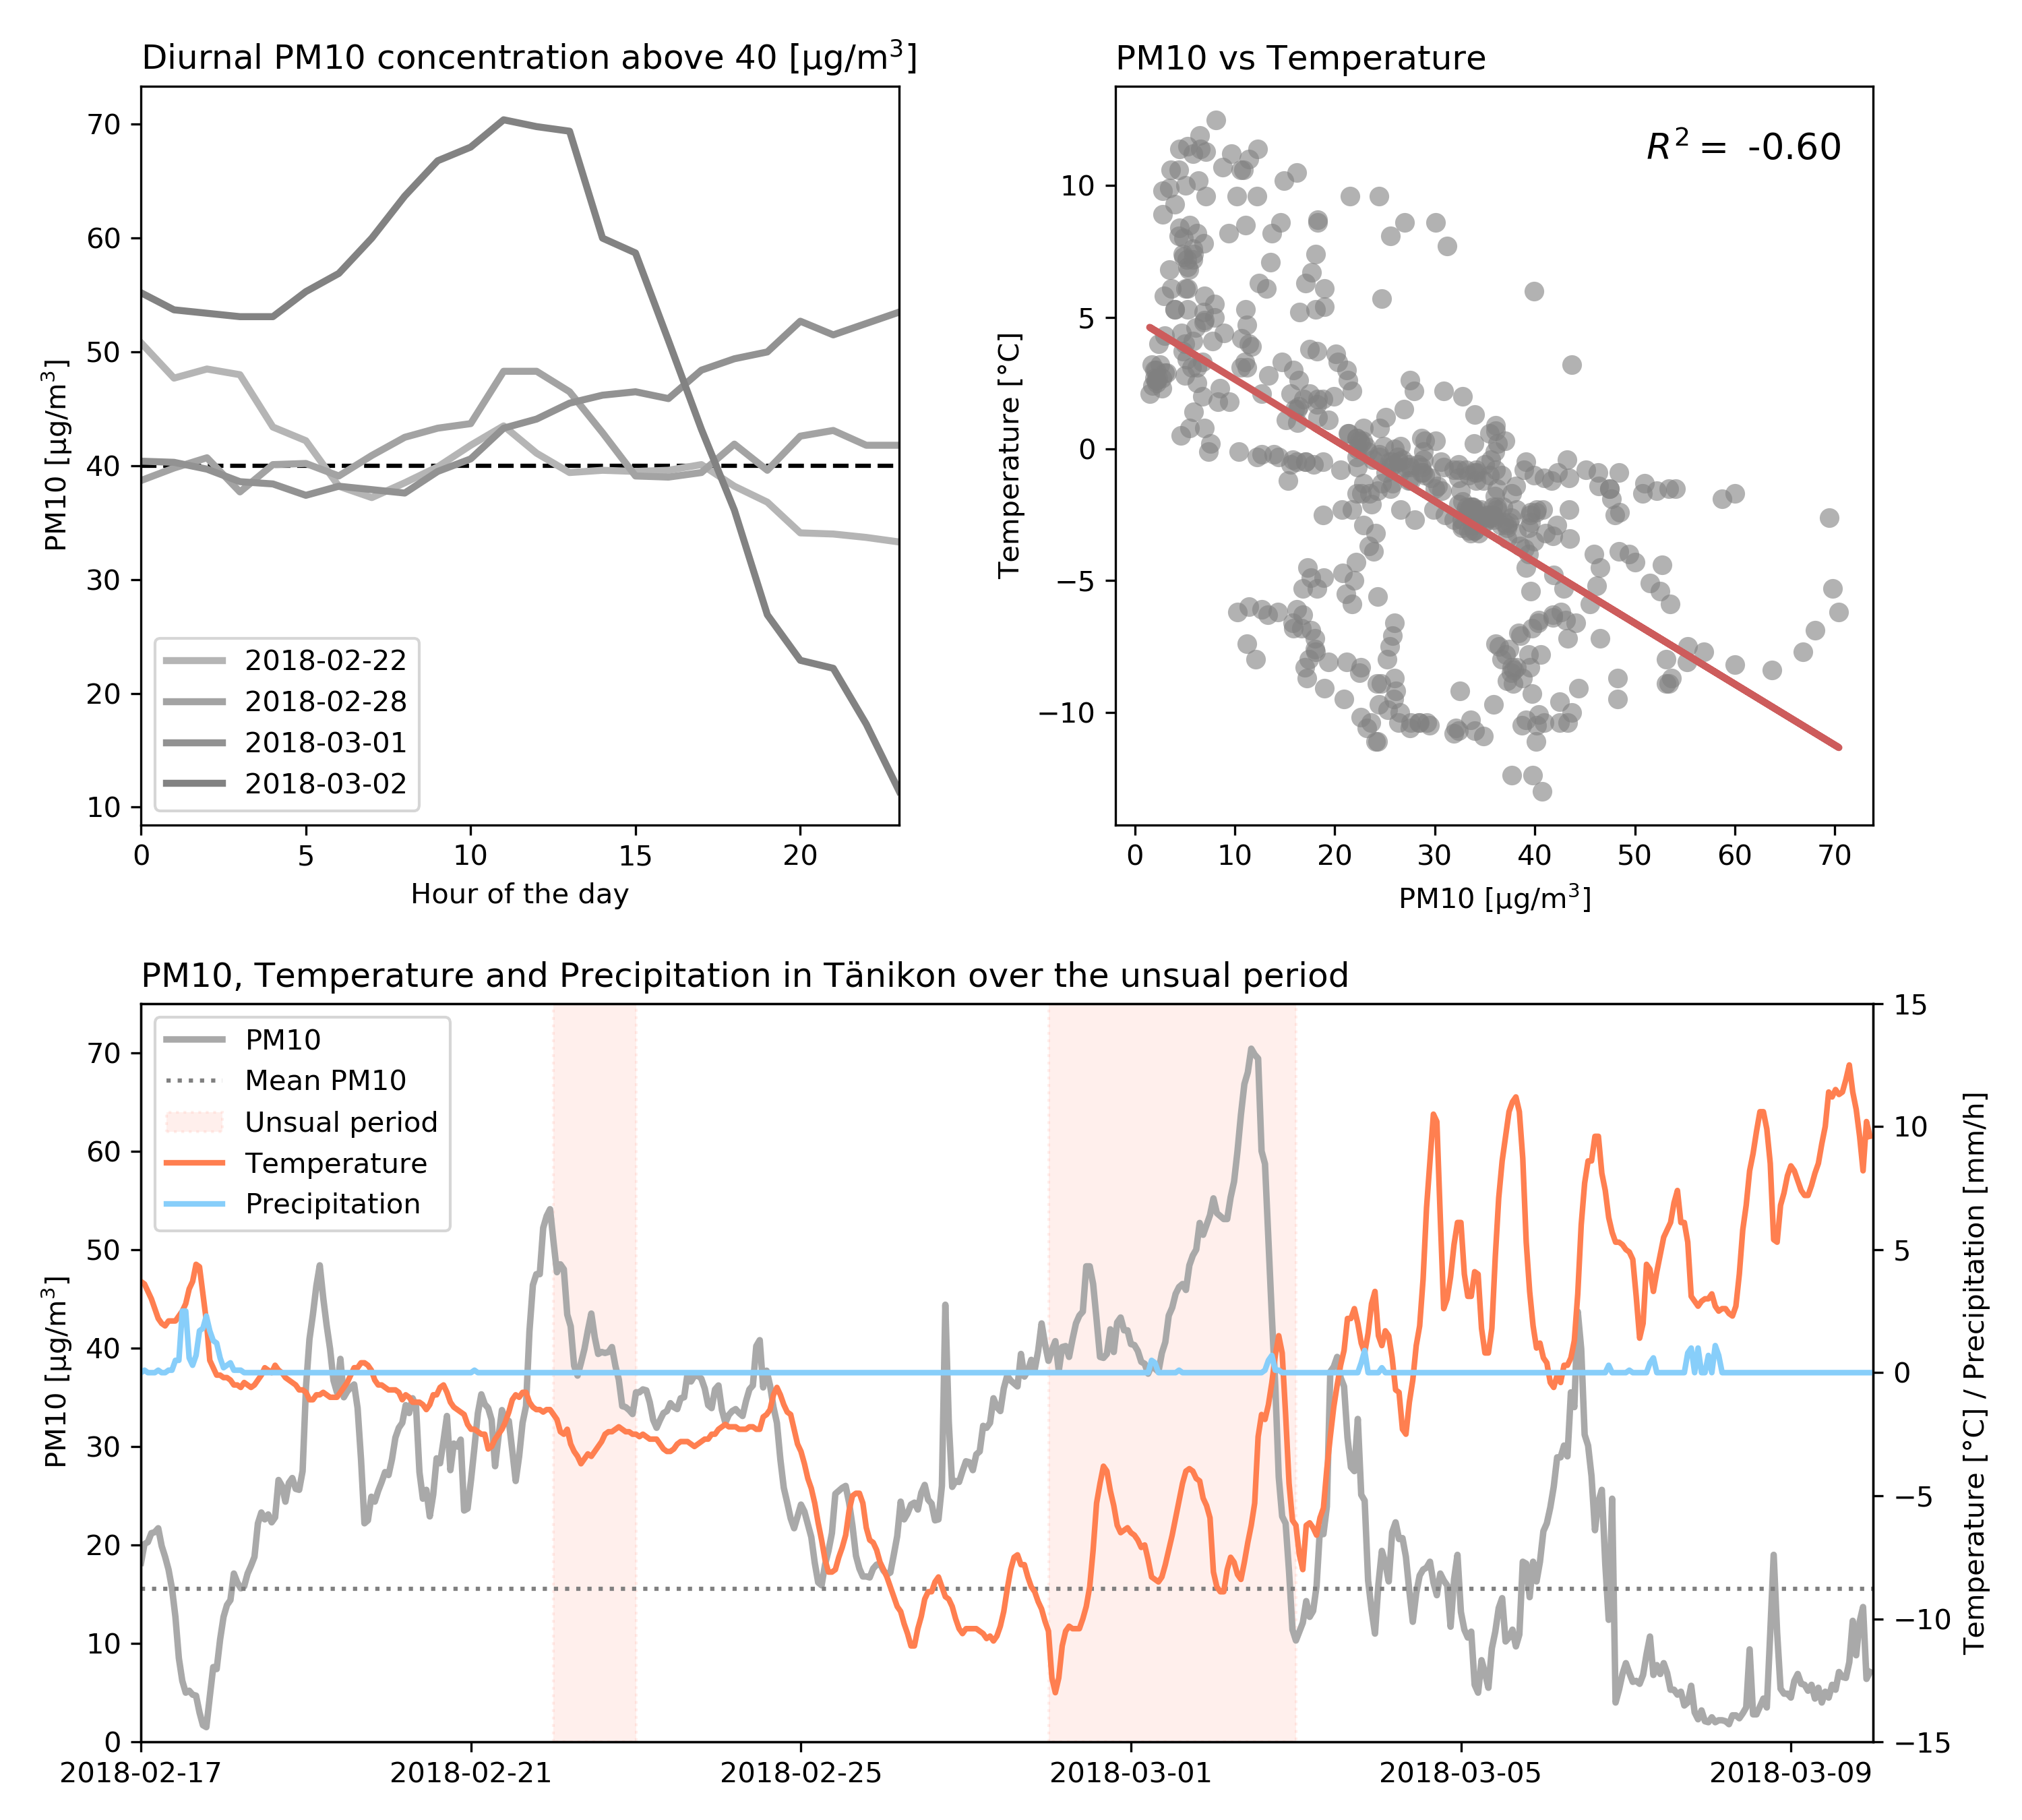
\includegraphics[width = 1 \textwidth]{Figures/UnsualPeriodPM10Tanikon.png}
        \caption{\textbf{Analysis of PM10 between 17.02.18 and 04.03.18 in Tänikon.} The top left plot presents the diurnal evolution of the four days exceeding 40 [\textmu g/m\textsuperscript{3}] on a daily average. The top right plot shows the temperature in function of the PM10 concentration over the period spanning from 17.02.18 to the 04.03.05. The red line is a linear fit to those points. The bottom plot present the time-series over the unusual period for the PM10, the temperature and the precipitation. The orange rectangles highlight the days where the daily PM10 exceeded 40 [\textmu g/m\textsuperscript{3}].}
        \label{fig:unusual-summary-plots}
    \end{figure}
    \\
    The qualitative observation of the time-series of the pollutants and meteorological parameters during this period shows that the temperature is rather low during the \textit{unusual period} as it reached -10 [\degree C]. The PM10 decreases as the temperature goes up. It suggests a negative correlation between PM10 and temperature. In consequence, it is supposed that PM10 and temperature are linked. The time-series of precipitation also suggest that precipitation lowers PM10. In consequence, the correlation between temperature and PM10 might not be perfect as PM10 seems to depend on many variables. The bottom plot of figure \ref{fig:unusual-summary-plots} shows the PM10, temperature and precipitation time-series during the unusual period with the days above 40 [\textmu g/m\textsuperscript{3}] highlighted by the orange rectangles. 
    \\
    \\
    In a similar fashion, a one-tailed Mann-Whitney-U test is performed to assess whether the temperature mean during the unusual period is lower than the mean over the winter season. It thus tests : \textit{H : \textmu \textsubscript{T unusual period} = \textmu \textsubscript{T winter}} against \textit{A : \textmu \textsubscript{T unusual period} $<$ \textmu \textsubscript{T winter}}. The null hypothesis is significantly rejected with a p-value of 4.155$\cdot$10\textsuperscript{-168}. Therefore, the temperature is significantly lower during the unusual period. 
    \\
    In a second step, the scatter-plot of PM10 vs Temperature (top right plot on figure \ref{fig:unusual-summary-plots}) together with the good negative Pearson correlation coefficient (R\textsuperscript{2} = -0.60) supports the hypothesis that temperature and PM10 are inversely linked over the unusual period. 
    \\
    \\
    However, a good correlation does not necessarily imply a causation between the two variables and there might be some confounding variables. It thus requires to explore what might cause this correlation between temperature and PM10. 
    \\
    \\
    In the first place a direct link between the two variables is explored. The atmospheric air can be considered as a ideal gas, and therefore it follows PV = nRT. The concentration can be represented as C = n/V which leads to the following relation C = P$\cdot$(RT)\textsuperscript{-1}. In consequence C $\propto$ T\textsuperscript{-1}. It means that at high temperature, the concentration will be smaller as the air expands and inversely, at low temperature, the concentration will increase as the air compress itself.
    \\
    \\
    Seconly, an indirect antropogenic link is explored. Indeed Tänikon is a rural area grouping many habitations. A decrease in outdoor temperature will push inhabitants to increase the heating of their households through a combustion at higher rate (chimney wood burning or fuel heater). An increased combustion would emit more PM10 in the village.  
    \\
    \\
    In brief, the combination of both physical and antropogenic link may be the reason for this unusual increases of PM10 during the unusual cold period of February 2018 \cite{meteoSuisse_Feb2018}. 

\section{Conclusion}
    In conclusion, it turns out that the nitrogen oxide concentrations are changing statistically (p-values $\approx$ 0) between week-end and week-days in both Sion and Tänikon. Therefore, we can conclude that antropogenic activities are significantly influencing the nitrogen oxide concentration. However, ozone does not seem to be significantly different between week-end and week-days at both locations. This result suggests that the ozone production is not, or only poorly negatively correlated with NO\textsubscript{x}. 
    \\
    \\
    Moreover, the effect of temperature and radiation on ozone production have been highlighted through the correlation analysis which has shown a strong positive correlation between these variables. The results suggests that solar radiation is the main cause of ozone increase with a lag of 3h (where it yields the highest correlation). 
    \\
    \\
    In addition, the emission source analysis suggests that the hourly measures of NO\textsubscript{2} are log-normally distributed and can thus be understood as a point source in Sion but not in Tänikon. The point source nature in Sion is explained by the proximity of the highway as a major emission source. It also seems that PM10 may be seen as a point source in Sion but not in Tänikon. This is potentially due to a gravel quarry situated south-west of the measurement station. 
    \\
    \\
    Finally, the unusual PM10 increase in Tänikon during February 2018 has been explained by the lowering of temperature (below -10 [\degree C]) and the induced increase of heating activity in the habitation surrounding of the measurement station. 

\newpage
\bibliographystyle{unsrt}
\bibliography{references}

\end{document}